\documentclass[12pt]{ociamthesis}  % default square logo
%\documentclass[12pt,beltcrest]{ociamthesis} % use old belt crest logo
%\documentclass[12pt,shieldcrest]{ociamthesis} % use older shield crest logo

%load any additional packages
\usepackage{amssymb}
\usepackage{listings}

%input macros (i.e. write your own macros file called mymacros.tex
%and uncomment the next line)
%\include{mymacros}

\title{Modul Praktikum \\[1ex]     %your thesis title,
        Kecerdasan Buatan}   %note \\[1ex] is a line break in the title

\author{Rolly Maulana Awangga}             %your name
\college{0410118609\\[5ex]
Applied Bachelor of Informatics Engineering}  %your college

%\renewcommand{\submittedtext}{change the default text here if needed}
\degree{Politeknik Pos Indonesia}     %the degree
\degreedate{Bandung 2019}         %the degree date

%end the preamble and start the document
\begin{document}

%this baselineskip gives sufficient line spacing for an examiner to easily
%markup the thesis with comments
\baselineskip=18pt plus1pt

%set the number of sectioning levels that get number and appear in the contents
\setcounter{secnumdepth}{3}
\setcounter{tocdepth}{3}


\maketitle                  % create a title page from the preamble info
\include{section/dedication}        % include a dedication.tex file
\include{section/acknowlegements}   % include an acknowledgements.tex file
\include{section/abstract}          % include the abstract

\begin{romanpages}          % start roman page numbering
\tableofcontents            % generate and include a table of contents
\listoffigures              % generate and include a list of figures
\end{romanpages}            % end roman page numbering

%now include the files of latex for each of the chapters etc
\chapter{Mengenal Kecerdasan Buatan dan ScikitLearn}

\section{Teori}

\subsection{Kecerdasan Buatan}
RESUME 1

\paragraph{Definisi}\hspace{0pt} \par
Kecerdasan Buatan adalah kemampuan komputer digital atau robot yang dikendalikan komputer untuk melakukan tugas yang umumnya dikaitkan dengan sesuatu yang cerdas. Istilah ini sering diterapkan pada proyek pengembangan sistem yang diberkahi dengan karakteristik proses intelektual manusia, seperti kemampuan untuk berpikir, menemukan makna, menggeneralisasi, atau belajar dari pengalaman masa lalu.

\paragraph{Sejarah Singkat}\hspace{0pt}\par
Pada awal 50-an, studi tentang "mesin bepikir" memiliki berbagai nama seperti cybernetics, teori automata, dan pemrosesan informasi. Pada tahun 1956, para ilmuwan jenius seperti Alan Turing, Norbert Wiener, Claude Shannon dan Warren McCullough telah bekerja secara independen di bidang cybernetics, matematika, algoritma dan teori jaringan.
Namun, seorang ilmuwan komputer dan kognitif John McCarthy adalah orang yang datang dengan ide untuk bergabung dengan upaya penelitian terpisah ini ke dalam satu bidang yang akan mempelajari topik baru untuk imajinasi manusia yaitu Kecerdasan Buatan. Dia adalah orang yang menciptakan istilah tersebut dan kemudian mendirikan laboratorium Kecerdasan Buatan di MIT dan Stanford.
Pada tahun 1956, McCarthy yang sama mendirikan Konferensi Dartmouth di Hanover, New Hampshire. Peneliti terkemuka dalam teori kompleksitas, simulasi bahasa, hubungan antara keacakan dan pemikiran kreatif, jaringan saraf diundang. Tujuan dari bidang penelitian yang baru dibuat adalah untuk mengembangkan mesin yang dapat mensimulasikan setiap aspek kecerdasan. Itulah sebabnya Konferensi Dartmouth 1956 dianggap sebagai kelahiran Kecerdasan Buatan.
Sejak itu, Kecerdasan Buatan telah hidup melalui dekade kemuliaan dan cemoohan, yang dikenal luas sebagai musim panas dan musim dingin AI. Musim panasnya ditandai dengan optimisme dan dana besar, sedangkan musim dinginnya dihadapkan dengan pemotongan dana, ketidakpercayaan dan pesimisme.

\paragraph{Perkembangan Kecerdasan Buatan}\hspace{0pt} \par
AI Summer 1 [1956-1973]
Konferensi Dartmouth diikuti oleh 17 tahun kemajuan luar biasa. Proyek penelitian yang dilakukan di MIT, universitas di Edinburgh, Stanford dan Carnegie Mellon menerima dana besar-besaran, yang akhirnya membuahkan hasil.
Selama tahun-tahun itulah komputer pemrograman mulai melakukan masalah aljabar, membuktikan teorema geometris, memahami dan menggunakan sintaks dan tata bahasa Inggris. Terlepas dari ditinggalkannya koneksionisme dan terjemahan mesin yang gagal, yang menunda penelitian Natural Language Processing (NLP) selama bertahun-tahun, banyak prestasi dari masa lalu yang membuat sejarah. Berikut ini beberapa di antaranya:
Pelopor pembelajaran mesin, Ray Solomonoff meletakkan dasar-dasar teori matematika AI, memperkenalkan metode Bayesian universal untuk inferensi dan prediksi induktif Thomas Evans menciptakan program ANALOGI heuristik, yang memungkinkan komputer memecahkan masalah geometri-analogi Unimation, perusahaan robotika pertama di dunia, menciptakan robot industri Unimate, yang bekerja pada jalur perakitan mobil General Motors. Joseph Weizenbaum membangun ELIZA - program interaktif yang dapat membawa percakapan dalam bahasa Inggris tentang topik apa pun.Ross Quillian menunjukkan jaring semantik, sedangkan Jaime Carbonell (Sr.) mengembangkan Cendekia - program interaktif untuk instruksi yang dibantu komputer berdasarkan jaring semantik. Edward Feigenbaum dan Julian Feldman menerbitkan Computers and Thought, kumpulan artikel pertama tentang AI.
\subsection{Definisi}
RESUME 2

\paragraph{Supervised Learning}\hspace{0pt}  \par
Supervised Learning adalah tugas pengumpulan data untuk menyimpulkan fungsi dari data pelatihan berlabel. Data pelatihan terdiri dari serangkaian contoh pelatihan. Dalam supervised learningi, setiap contoh adalah pasangan yang terdiri dari objek input (biasanya vektor) dan nilai output yang diinginkan (juga disebut sinyal pengawasan super). Algoritma pembelajaran yang diawasi menganalisis data pelatihan dan menghasilkan fungsi yang disimpulkan, yang dapat digunakan untuk memetakan contoh-contoh baru. Skenario optimal akan memungkinkan algoritma menentukan label kelas dengan benar untuk instance yang tidak terlihat. Ini membutuhkan algoritma pembelajaran untuk menggeneralisasi dari data pelatihan untuk situasi yang tidak terlihat dengan cara yang “masuk akal”.
Supervised Learningi menyediakan algoritma pembelajaran dengan jumlah yang diketahui untuk mendukung penilaian di masa depan. Chatbots, mobil self-driving, program pengenalan wajah, sistem pakar dan robot adalah beberapa sistem yang dapat menggunakan pembelajaran yang diawasi atau tidak diawasi. Supervised Learning sebagian besar terkait dengan AI berbasis pengambilan tetapi mereka juga mungkin mampu menggunakan model pembelajaran generatif.
Data pelatihan untuk pembelajaran yang diawasi mencakup serangkaian contoh dengan subjek input berpasangan dan output yang diinginkan (yang juga disebut sebagai sinyal pengawasan). Dalam pembelajaran yang diawasi untuk pemrosesan gambar, misalnya, sistem AI mungkin dilengkapi dengan gambar berlabel kendaraan dalam kategori seperti mobil dan truk. Setelah jumlah pengamatan yang cukup, sistem harus dapat membedakan antara dan mengkategorikan gambar yang tidak berlabel, di mana waktu pelatihan dapat dikatakan lengkap.
Model Supervised Learning memiliki beberapa keunggulan dibandingkan pendekatan tanpa pengawasan, tetapi mereka juga memiliki keterbatasan. Sistem lebih cenderung membuat penilaian bahwa manusia dapat berhubungan, misalnya, karena manusia telah memberikan dasar untuk keputusan. Namun, dalam kasus metode berbasis pengambilan, Supervised Learning mengalami kesulitan dalam menangani informasi baru. Jika suatu sistem dengan kategori untuk mobil dan truk disajikan dengan sepeda, misalnya, ia harus salah dikelompokkan dalam satu kategori atau yang lain. Namun, jika sistem AI bersifat generatif, ia mungkin tidak tahu apa sepeda itu tetapi akan dapat mengenalinya sebagai milik kategori yang terpisah.

\paragraph{Regresi}\hspace{0pt} \par
Regresi adalah membahas masalah ketika variabel output adalah nilai riil atau berkelanjutan, seperti "gaji" atau "berat". Banyak model yang berbeda dapat digunakan, yang paling sederhana adalah regresi linier. Ia mencoba untuk menyesuaikan data dengan hyper-plane terbaik yang melewati poin.

\paragraph{Klasifikasi}\hspace{0pt} \par
Dalam masalah klasifikasi, kami mencoba memprediksi sejumlah nilai terpisah. Label (y) umumnya datang dalam bentuk kategorikal dan mewakili sejumlah kelas. Dalam pembelajaran mesin dan statistik, klasifikasi adalah pendekatan pembelajaran yang diawasi di mana program komputer belajar dari input data yang diberikan kepadanya dan kemudian menggunakan pembelajaran ini untuk mengklasifikasikan pengamatan baru. Kumpulan data ini mungkin hanya bersifat dua kelas (seperti mengidentifikasi apakah orang tersebut berjenis kelamin laki-laki atau perempuan atau bahwa surat itu spam atau bukan-spam) atau mungkin juga multi-kelas. Beberapa contoh masalah klasifikasi adalah: pengenalan ucapan, pengenalan tulisan tangan, identifikasi metrik, klasifikasi dokumen dll.

\paragraph{Unsupervised Learning}\hspace{0pt} \par
Unsupervised Learning adalah pelatihan algoritma kecerdasan buatan (AI) menggunakan informasi yang tidak diklasifikasikan atau diberi label dan memungkinkan algoritma untuk bertindak atas informasi tersebut tanpa bimbingan.
Dalam Unsupervised Learning, sistem AI dapat mengelompokkan informasi yang tidak disortir berdasarkan persamaan dan perbedaan meskipun tidak ada kategori yang disediakan. Sistem AI yang mampu pembelajaran tanpa pengawasan sering dikaitkan dengan model pembelajaran generatif, meskipun mereka juga dapat menggunakan pendekatan berbasis pengambilan (yang paling sering dikaitkan dengan pembelajaran yang diawasi). Chatbots, mobil yang bisa mengemudi sendiri, program pengenalan wajah, sistem pakar dan robot adalah beberapa sistem yang dapat menggunakan pendekatan pembelajaran yang diawasi atau tidak terawasi.
Dalam Unsupervised Learning, sistem AI disajikan dengan data yang tidak berlabel, tidak terkategorisasi dan algoritma sistem bekerja pada data tanpa pelatihan sebelumnya. Outputnya tergantung pada algoritma kode. Menundukkan suatu sistem pada Unsupervised Learning adalah salah satu cara untuk menguji AI.
Algoritma Unsupervised Learning dapat melakukan tugas pemrosesan yang lebih kompleks daripada sistem pembelajaran yang diawasi. Namun, pembelajaran tanpa pengawasan bisa lebih tidak terduga daripada model alternatif. Sementara Unsupervised Learningi mungkin, misalnya, mencari tahu sendiri cara memilah kucing dari anjing, mungkin juga menambahkan kategori yang tidak terduga dan tidak diinginkan untuk menangani breed yang tidak biasa, membuat kekacauan bukannya keteraturan.

\paragraph{Data Set}\hspace{0pt} \par
mendapatkan data yang tepat berarti mengumpulkan atau mengidentifikasi data yang berkorelasi dengan hasil yang ingin Anda prediksi; yaitu data yang berisi sinyal tentang peristiwa yang Anda pedulikan. Data harus diselaraskan dengan masalah yang Anda coba selesaikan. Gambar kucing tidak terlalu berguna ketika Anda sedang membangun sistem identifikasi wajah. Memverifikasi bahwa data selaras dengan masalah yang ingin Anda selesaikan harus dilakukan oleh ilmuwan data. Jika Anda tidak memiliki data yang tepat, maka upaya Anda untuk membangun solusi AI harus kembali ke tahap pengumpulan data.
Format ujung kanan untuk pembelajaran dalam umumnya adalah tensor, atau array multi-dimensi. Jadi jalur pipa data yang dibangun untuk pembelajaran mendalam umumnya akan mengkonversi semua data - baik itu gambar, video, suara, suara, teks atau deret waktu - menjadi vektor dan tensor yang dapat diterapkan operasi aljabar linier. Data itu seringkali perlu dinormalisasi, distandarisasi dan dibersihkan untuk meningkatkan kegunaannya, dan itu semua adalah langkah dalam ETL pembelajaran mesin. Deeplearning4j menawarkan alat ETV DataVec untuk melakukan tugas-tugas pemrosesan data tersebut.
Pembelajaran yang dalam, dan pembelajaran mesin yang lebih umum, membutuhkan pelatihan yang baik agar bekerja dengan baik. Mengumpulkan dan membangun set pelatihan - badan yang cukup besar dari data yang diketahui - membutuhkan waktu dan pengetahuan khusus domain tentang di mana dan bagaimana mengumpulkan informasi yang relevan. Perangkat pelatihan bertindak sebagai tolok ukur terhadap mana jaring pembelajaran dalam dilatih. Itulah yang mereka pelajari untuk direkonstruksi sebelum mereka melepaskan data yang belum pernah mereka lihat sebelumnya.
Pada tahap ini, manusia yang berpengetahuan luas perlu menemukan data mentah yang tepat dan mengubahnya menjadi representasi numerik yang dapat dipahami oleh algoritma pembelajaran mendalam, tensor. Membangun set pelatihan, dalam arti tertentu, pra-pra-pelatihan.
Set pelatihan yang membutuhkan banyak waktu atau keahlian dapat berfungsi sebagai keunggulan dalam dunia ilmu data dan pemecahan masalah. Sifat keahlian sebagian besar dalam memberi tahu algoritma Anda apa yang penting bagi Anda dengan memilih apa yang masuk ke dalam set pelatihan.
Ini melibatkan menceritakan sebuah kisah - melalui data awal yang Anda pilih - yang akan memandu jaring pembelajaran mendalam Anda saat mereka mengekstraksi fitur-fitur penting, baik di set pelatihan maupun dalam data mentah yang telah mereka ciptakan untuk dipelajari.
Untuk membuat set pelatihan yang bermanfaat, Anda harus memahami masalah yang Anda selesaikan; yaitu apa yang Anda inginkan agar jaring pembelajaran mendalam Anda memperhatikan, di mana hasil yang ingin Anda prediksi.

\paragraph{Training Set} \hspace{0pt} \par
Menjalankan pelatihan yang diatur melalui jaringan saraf mengajarkan pada net cara menimbang berbagai fitur, menyesuaikan koefisien berdasarkan kemungkinan mereka meminimalkan kesalahan dalam hasil Anda.
Koefisien-koefisien tersebut, juga dikenal sebagai parameter, akan terkandung dalam tensor dan bersama-sama mereka disebut model, karena mereka mengkodekan model data yang mereka latih. Mereka adalah takeaways paling penting yang akan Anda dapatkan dari pelatihan jaringan saraf.

\paragraph{Test Set} \hspace{0pt} \par
Ini berfungsi sebagai meterai persetujuan, dan Anda tidak menggunakannya sampai akhir. Setelah Anda melatih dan mengoptimalkan data Anda, Anda menguji jaringan saraf Anda terhadap pengambilan sampel acak akhir ini. Hasil yang dihasilkannya harus memvalidasi bahwa jaring Anda secara akurat mengenali gambar, atau mengenalinya setidaknya [x] dari jumlah tersebut. Jika Anda tidak mendapatkan prediksi yang akurat, kembalilah ke set pelatihan, lihat hyperparameter yang Anda gunakan untuk menyetel jaringan, serta kualitas data Anda dan lihat teknik pra-pemrosesan Anda.


\section{Instalasi}
Membuka https://scikit-learn.org/stable/tutorial/basic/tutorial.html. Dengan menggunakan bahasa yang mudah dimengerti dan bebas plagiat. 
Dan wajib skrinsut dari komputer sendiri.
\subsection{Instalasi library scikit dari anaconda, mencoba kompilasi dan uji coba ambil contoh kode dan lihat variabel explorer}
\begin{enumerate}
\item
Pastikan bahwa sudah terinstal Anaconda pada PC anda, caranya buka CMD lalu ketikan "conda --version" jika hasilnya seperti 
\begin{figure}
	\begin{center}
   	 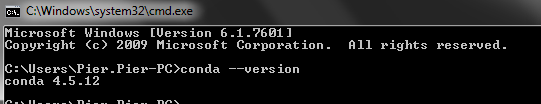
\includegraphics[scale=1]{figures/versiconda.png}
   	 \caption{Versi Anaconda Yang Digunakan}	
	\end{center}
\end{figure}
\item
Pastikan juga Kebutuhan Scikit seperti Numpy, Scipy dan Python telah terinstal. untuk mengeceknya buka CMD dan ketikan seperti gambar berikut.
\begin{figure}
	\begin{center}
   	 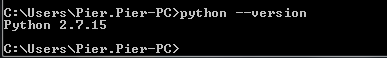
\includegraphics[scale=1]{figures/gambar.png}
   	 \caption{Versi Python Yang Digunakan}	
	\end{center}
\end{figure}
\item 
Pada CMD ketikan "conda install scikit-learn" kemudian tunggu sampai instalasi selesai.
\begin{figure}
	\begin{center}
   	 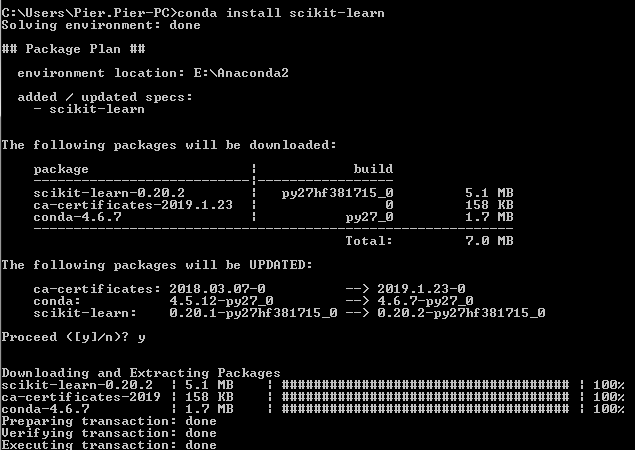
\includegraphics[scale=1]{figures/instalscikit.png}
   	 \caption{Instalasi Scikit Dari Anaconda}	
	\end{center}
\end{figure}
\item 
Setelah itu, kita akan mencoba salah satu contoh dasar penggunaan scikit pada website sebelumnya. Dan disini menggunakan contoh Multilabel classification.
\item 
Salin skrip contoh tersebut ke Text Editor Visual Code atau yang anda miliki. File ini kemudian di save dengan nama "contoh.py"
\begin{figure}
	\begin{center}
   	 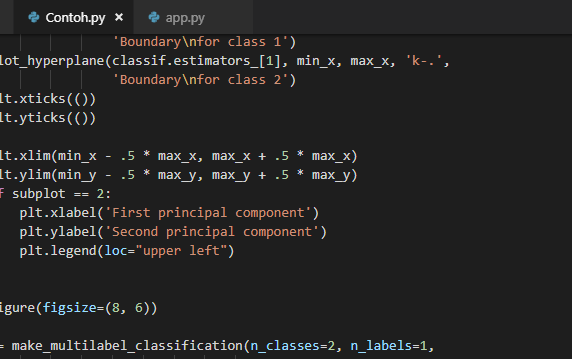
\includegraphics[scale=1]{figures/contoh.png}
   	 \caption{Contoh Skrip}	
	\end{center}
\end{figure}
\item 
Setelah tersimpan, jalankan di CMD dengan mengetikan "python contoh.py" maka akan muncul hasil seperti dibawah ini.
\begin{figure}
	\begin{center}
   	 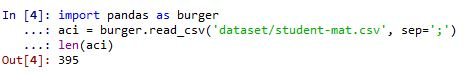
\includegraphics[scale=1]{figures/hasil1.png}
   	 \caption{Hasil Yang Muncul Di CMD}	
	\end{center}
\end{figure}
\begin{figure}
	\begin{center}
   	 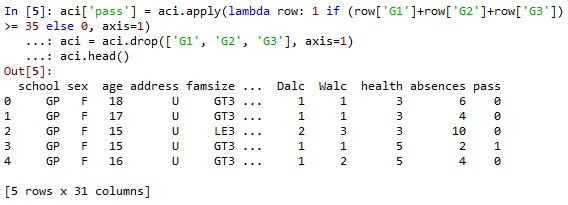
\includegraphics[scale=1]{figures/hasil2.png}
   	 \caption{Gambar Yang Muncul Dari Matplotlib}	
	\end{center}
\end{figure}
\end{enumerate}

\subsection{Mencoba Loading an example dataset, menjelaskan maksud dari tulisan tersebut dan mengartikan per baris}
\begin{enumerate}
\item
Mengimmport dataset, iris dan digit sebagai contoh data.
\begin{figure}
	\begin{center}
   	 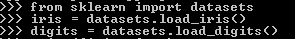
\includegraphics[scale=1]{figures/penjelasan1.png}
   	 \caption{Penjelasan }	
	\end{center}
\end{figure}
\item
Misalnya, dalam kasus dataset digit, digits.data memberikan akses ke fitur yang dapat digunakan untuk mengklasifikasikan sampel digit.
\begin{figure}
	\begin{center}
   	 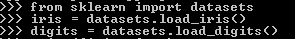
\includegraphics[scale=1]{figures/penjelasan1.png}
   	 \caption{Penjelasan 2}	
	\end{center}
\end{figure}
\item 
digit.target memberikan kebenaran dasar untuk dataset digit, yaitu angka yang sesuai dengan setiap gambar digit yang dipelajari.
\begin{figure}
	\begin{center}
   	 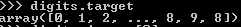
\includegraphics[scale=1]{figures/penjelasan3.png}
   	 \caption{Penjelasan 3}	
	\end{center}
\end{figure}
\item 
menggambarkan bagaimana mulai dari masalah awal seseorang dapat membentuk data untuk konsumsi di scikit-belajar.
\begin{figure}
	\begin{center}
   	 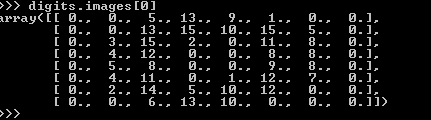
\includegraphics[scale=1]{figures/penjelasan4.png}
   	 \caption{Penjelasan 4}	
	\end{center}
\end{figure}

\end{enumerate}

\begin{enumerate}
\item
Mencoba Learning and predicting, menjelaskan maksud dari tulisan tersebut dan mengartikan per baris[hari ke 2](10)
\item
mencoba Model persistence, menjelaskan maksud dari tulisan tersebut dan mengartikan per baris[hari ke 2](10)
\item 
Mencoba Conventions, menjelaskan maksud dari tulisan tersebut dan mengartikan per baris[hari ke 2](10)
\end{enumerate}


\section{Penanganan Error}
Dari percobaan yang dilakukan di atas, apabila mendapatkan error maka:

\begin{enumerate}
	\item
	skrinsut error[hari ke 2](10)
	\item
Tuliskan kode eror dan jenis errornya [hari ke 2](10)
	\item
Solusi pemecahan masalah error tersebut[hari ke 2](10)

\end{enumerate}

\section{Teori}
Teori mencakup resume dari beberapa pembahasan. yaitu :
\begin{enumerate}
\begin
\item Definisi Kecerdasan Buatan.
\par Jadi yang dimaksud dengan  kecerdasan buatan yaitu  salah satu dari cabang Ilmu pengetahuan yang kita punya dan  berhubungan juga dengan pemanfaatan mesin yaitu untuk dapat memecahkan suatu  persoalan yang rumit dengan  menggunakan cara yang lebih manusiawi.
\par Jadi yang dimaksud dengan supervised learning  adalah pembelajaran mesin yang diawasi menciptakan model yang melancarkan prediksi berdasarkan bukti adanya ketidakpastian. Algoritma pembelajaran yang diawasi memerlukan seperangkat data masukan dan tanggapan yang diketahui terhadap data (output) dan melatih model untuk menghasilkan prediksi yang masuk akal untuk respon terhadap data baru. Sedangkan untuk klasifikasi yaitu nilai output yang  bernilai diskrit (kelas) dan Bertujuan mengklasifikasi data baru dengan akurat diawasi dengan menggunakan teknik klasifikasi dan regresi untuk mengembangkan model prediktif. Yang dimaksud dengan regresi adlah nilai output yang bernilai kontinu (riil), Bertujuan memprediksi output dengan akurat untuk data baru.
\par Unsupervised learning tidak menggunakan data latih atau data training untuk melakukan prediksi maupun klasifikasi. Berdasarkan model matematisnya, algoritma ini tidak memiliki target variabel. Salah satu tujuan dari algoritma ini adalah mengelompokkan objek yang hampir sama dalam suatu area tertentu. Dan yang dimaksud dengan  Dataset adalah objek yang merepresentasikan data dan relasinya di memory. Strukturnya mirip dengan data di database. Dataset berisi koleksi dari datatable dan datarelation. Sedangkan testing set digunakan untuk mengukur sejauh mana classifier berhasil melakukan klasifikasi dengan benar. Dan training set digunakan oleh algoritma klassifikasi untuk membentuk sebuah model classifier. Model yang dimaksud ini merupakan representasi pengetahuan yang akan digunakan untuk prediksi kelas data baru yang belum pernah ada.
\end{enumerate} 


\chapter{Related Works}

Your related works, and your purpose and contribution which.
\section{Tasya Wiendhyra/1164086}
\subsection{binary classification dilengkapi ilustrasi gambar}
\begin{enumerate}
\item Binary classification yaitu berupa kelas positif dan kelas negatif. Klasifikasi biner adalah dikotomisasi yang diterapkan untuk tujuan praktis, dan dalam banyak masalah klasifikasi biner praktis, kedua kelompok tidak simetris - daripada akurasi keseluruhan, proporsi relatif dari berbagai jenis kesalahan yang menarik. Misalnya, dalam pengujian medis, false positive (mendeteksi penyakit ketika tidak ada) dianggap berbeda dari false negative (tidak mendeteksi penyakit ketika hadir).
\begin{figure}[ht]
\centering
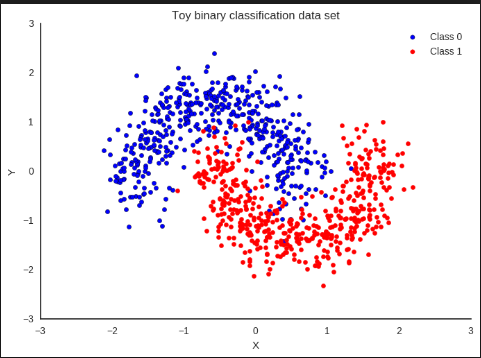
\includegraphics[scale=0.5]{figures/wiendh1.png}
\caption{Binary Classification}
\label{contoh}
\end{figure}
\end{enumerate}

\subsection{supervised learning dan unsupervised learning dan clustering dengan ilustrasi gambar}
\begin{enumerate}
\item Supervised learning adalah tugas pembelajaran mesin untuk mempelajari suatu fungsi yang memetakan input ke output berdasarkan contoh pasangan input-output. Ini menyimpulkan fungsi dari data pelatihan berlabel yang terdiri dari serangkaian contoh pelatihan. Dalam pembelajaran yang diawasi, setiap contoh adalah pasangan yang terdiri dari objek input (biasanya vektor) dan nilai output yang diinginkan (juga disebut sinyal pengawas). Algoritma pembelajaran yang diawasi menganalisis data pelatihan dan menghasilkan fungsi yang disimpulkan, yang dapat digunakan untuk memetakan contoh-contoh baru. Skenario optimal akan memungkinkan algoritma menentukan label kelas dengan benar untuk instance yang tidak terlihat. Ini membutuhkan algoritma pembelajaran untuk menggeneralisasi dari data pelatihan untuk situasi yang tidak terlihat dengan cara yang "masuk akal" (lihat bias induktif). Tugas paralel dalam psikologi manusia dan hewan sering disebut sebagai pembelajaran konsep. Contoh dibawah yaitu Supervised Learning dengan SVC.
\begin{figure}[ht]
\centering
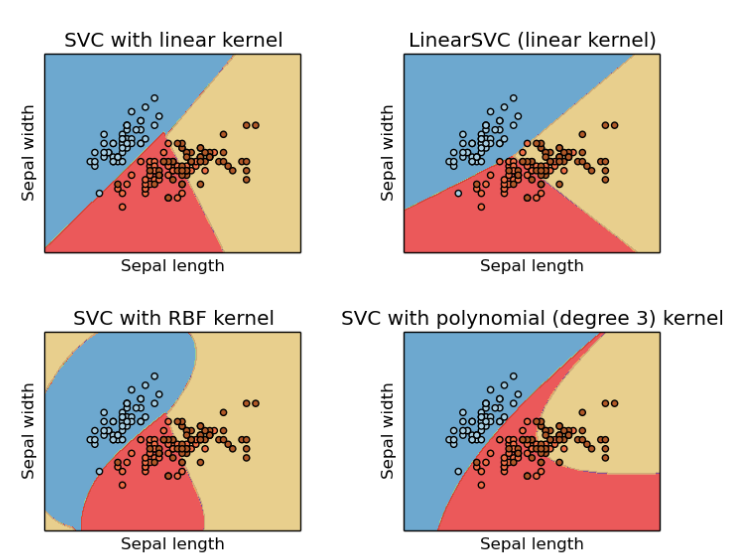
\includegraphics[scale=0.5]{figures/wiendh2.png}
\caption{Supervised Learning}
\label{contoh}
\end{figure}
\item Unsupervised learning adalah istilah yang digunakan untuk pembelajaran bahasa Ibrani, yang terkait dengan pembelajaran tanpa guru, juga dikenal sebagai organisasi mandiri dan metode pemodelan kepadatan probabilitas input. Analisis cluster sebagai cabang pembelajaran mesin yang mengelompokkan data yang belum diberi label, diklasifikasikan atau dikategorikan. Alih-alih menanggapi umpan balik, analisis klaster mengidentifikasi kesamaan dalam data dan bereaksi berdasarkan ada tidaknya kesamaan di setiap potongan data baru. BErikut merupakan contoh Unsupervised Learning dengan Gaussian mixture models.
\begin{figure}[ht]
\centering
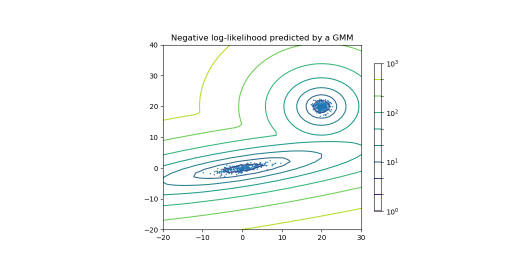
\includegraphics[scale=0.5]{figures/wiendh3.png}
\caption{Unsupervised Learning}
\label{contoh}
\end{figure}
\item Cluster analysis or clustering adalah tugas pengelompokan sekumpulan objek sedemikian rupa sehingga objek dalam kelompok yang sama (disebut klaster) lebih mirip (dalam beberapa hal) satu sama lain daripada pada kelompok lain (kluster). Ini adalah tugas utama penambangan data eksplorasi, dan teknik umum untuk analisis data statistik, yang digunakan di banyak bidang, termasuk pembelajaran mesin, pengenalan pola, analisis gambar, pengambilan informasi, bioinformatika, kompresi data, dan grafik komputer. Analisis Cluster sendiri bukan merupakan salah satu algoritma spesifik, tetapi tugas umum yang harus dipecahkan. Ini dapat dicapai dengan berbagai algoritma yang berbeda secara signifikan dalam pemahaman mereka tentang apa yang merupakan sebuah cluster dan bagaimana cara menemukannya secara efisien. Gagasan populer mengenai cluster termasuk kelompok dengan jarak kecil antara anggota cluster, area padat ruang data, interval atau distribusi statistik tertentu. Clustering karena itu dapat dirumuskan sebagai masalah optimasi multi-objektif. Algoritma pengelompokan dan pengaturan parameter yang sesuai (termasuk parameter seperti fungsi jarak yang akan digunakan, ambang kepadatan atau jumlah cluster yang diharapkan) tergantung pada set data individual dan penggunaan hasil yang dimaksudkan. Analisis kluster bukan merupakan tugas otomatis, tetapi proses berulang penemuan pengetahuan atau optimasi multi-objektif interaktif yang melibatkan percobaan dan kegagalan. Seringkali diperlukan untuk memodifikasi praproses data dan parameter model hingga hasilnya mencapai properti yang diinginkan.
\begin{figure}[ht]
\centering
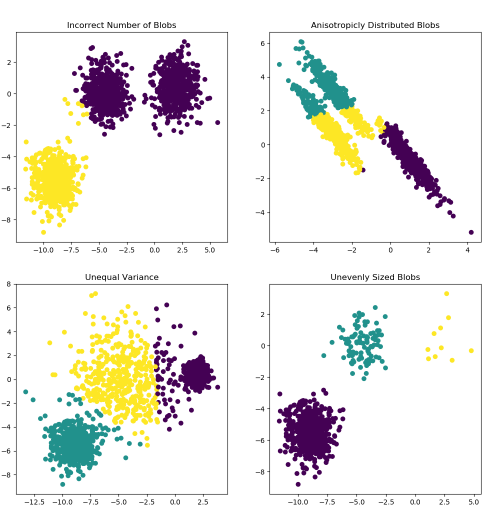
\includegraphics[scale=0.5]{figures/wiendh4.png}
\caption{Cluster}
\label{contoh}
\end{figure}
\end{enumerate}

\subsection{evaluasi dan akurasi dari buku dan disertai ilustrasi contoh
dengan gambar}
\begin{enumerate}
\item Evaluasi adalah tentang  bagaimana kita dapat mengevaluasi seberapa baik model bekerja dengan mengukur akurasinya. Dan akurasi akan didefinisikan sebagai persentase kasus yang diklasifikasikan dengan benar. Kita dapat menganalisis kesalahan yang dibuat oleh model, atau tingkat kebingungannya, menggunakan matriks kebingungan. Matriks kebingungan mengacu pada kebingungan dalam model, tetapi matriks kebingungan ini bisa menjadi sedikit sulit untuk dipahami ketika mereka menjadi sangat besar.
\begin{figure}[ht]
\centering
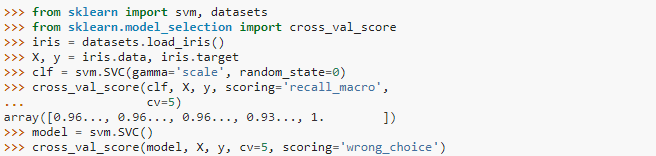
\includegraphics[scale=0.5]{figures/wiendh9.png}
\caption{ Evaluasi dan Akurasi}
\label{contoh}
\end{figure}
\end{enumerate}

\subsection{ bagaimana cara membuat dan membaca confusion matrix, buat confusion matrix }
\begin{enumerate}
\item Cara membuat dan membaca confusion matrix :
\begin{itemize}
\item 1)	Tentukan pokok permasalahan dan atributanya, misal gaji dan listik.
\item 2)	Buat pohon keputusan
\item 3)	Lalu data testingnya
\item 4)	Lalu mencari nilai a, b, c, dan d. Semisal a = 5, b = 1, c = 1, dan d = 3.
\item 5)	Selanjutnya mencari nilai recall, precision, accuracy, serta dan error rate.
\end{itemize}
\item Berikut adalah contoh dari confusion matrix :
\begin{itemize}
\item Recall =3/(1+3) = 0,75
\item Precision = 3/(1+3) = 0,75
\item Accuracy =(5+3)/(5+1+1+3) = 0,8
\item Error Rate =(1+1)/(5+1+1+3) = 0,2
\end{itemize}
\end{enumerate}

\subsection{bagaimana K-fold cross validation bekerja dengan gambar ilustrasi}
\begin{enumerate}
\item Cara kerja K-fold cross validation :
\begin{itemize}
\item 1)	Total instance dibagi menjadi N bagian.
\item 2)	Fold yang pertama adalah bagian pertama menjadi data uji (testing data) dan sisanya menjadi training data.
\item 3)	Lalu hitung akurasi berdasarkan porsi data tersebut dengan menggunakan persamaan.
\item 4)	Fold yang ke dua adalah bagian ke dua menjadi data uji (testing data) dan sisanya training data. 
\item 5)	Kemudian hitung akurasi berdasarkan porsi data tersebut.
\item 6)	Dan seterusnya hingga habis mencapai fold ke-K.
\item 7)	Terakhir hitung rata-rata akurasi K buah.
\end{itemize}
\begin{figure}[ht]
\centering
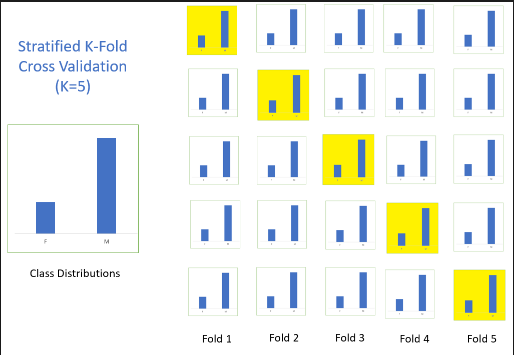
\includegraphics[scale=0.5]{figures/wiendh5.png}
\caption{K-fold cross validation }
\label{contoh}
\end{figure}
\end{enumerate}

\subsection{decision tree dengan gambar ilustrasi}
\begin{enumerate}
\item Decision Tree dalah metode pembelajaran yang diawasi non-parametrik yang digunakan untuk klasifikasi dan regresi. Tujuannya adalah untuk membuat model yang memprediksi nilai variabel target dengan mempelajari aturan keputusan sederhana yang disimpulkan dari fitur data.\\
Misalnya, dalam contoh di bawah ini, decision tree belajar dari data untuk memperkirakan kurva sinus dengan seperangkat aturan keputusan if-then-else. Semakin dalam pohon, semakin rumit aturan keputusan dan semakin bugar modelnya.
\begin{figure}[ht]
\centering
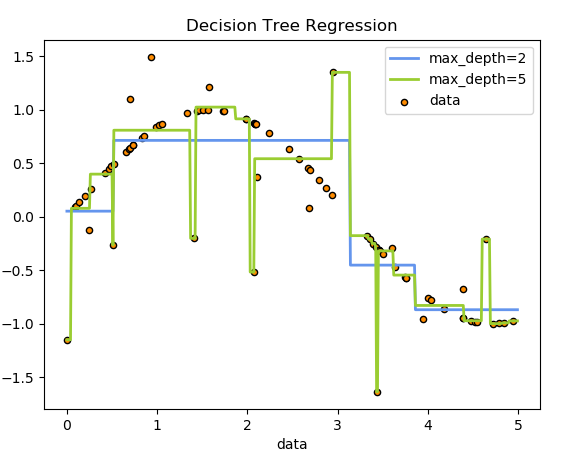
\includegraphics[scale=0.5]{figures/wiendh6.png}
\caption{Decision Tree}
\label{contoh}
\end{figure}
\end{enumerate}

\subsection{Information Gain dan entropi dengan gambar ilustrasi}
\begin{enumerate}
\item Information gain didasarkan pada penurunan entropi setelah dataset dibagi pada atribut. Membangun decision tree adalah semua tentang menemukan atribut yang mengembalikan perolehan informasi tertinggi (mis., Cabang yang paling homogen).
\begin{figure}[ht]
\centering
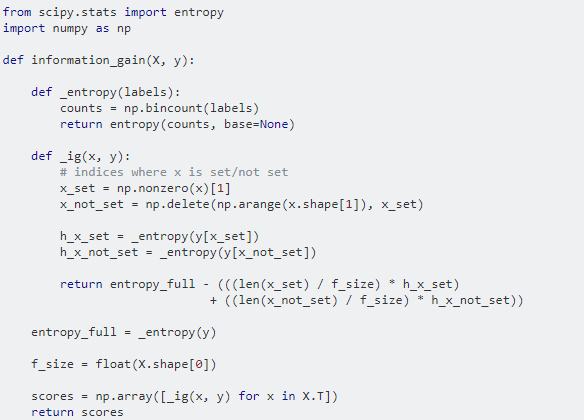
\includegraphics[scale=0.5]{figures/wiendh7.png}
\caption{Information gain}
\label{contoh}
\end{figure}
\item Entropi adalah ukuran keacakan dalam informasi yang sedang diproses. Semakin tinggi entropi, semakin sulit untuk menarik kesimpulan dari informasi itu. Membalik koin adalah contoh tindakan yang memberikan informasi yang acak. Untuk koin yang tidak memiliki afinitas untuk kepala atau ekor, hasil dari sejumlah lemparan sulit diprediksi. Mengapa? Karena tidak ada hubungan antara membalik dan hasilnya. Inilah inti dari entropi.
\begin{figure}[ht]
\centering
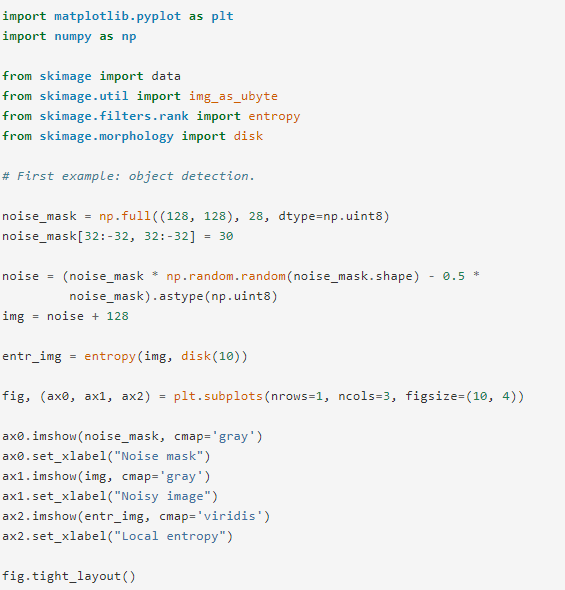
\includegraphics[scale=0.5]{figures/wiendh8.png}
\caption{Entropi}
\label{contoh}
\end{figure}
\end{enumerate}


 
\chapter{Methods}

\section{The data}
PLease tell where is the data come from, a little brief of company can be put here.

\section{Method 1}
Definition, steps, algoritm or equation of method 1 and how to apply into your data
\section{Method 2}
Definition, steps, algoritm or equation of method 2 and how to apply into your data

\section{ANNISA FATHORONI/1164067}
\subsection{Teori}
Penyelesaian Tugas Harian 5 ( No. 1-6 )
\begin{enumerate}
\item Random Forest Dan Ilustrasi Gambarnya
\begin{itemize}
\item Pengertian Random Forest:

Random forests atau random decision forests adalah metode pembelajaran ensembel untuk klasifikasi, regresi dan tugas-tugas lain yang beroperasi dengan membangun banyak pohon keputusan pada waktu pelatihan dan menghasilkan kelas yang merupakan mode kelas (klasifikasi) atau prediksi rata-rata (regresi) dari masing-masing pohon. Random decision forests tepat untuk kebiasaan pohon keputusan 'overfitting' pada set pelatihan mereka.

\item Ilustrasi Gambar Random Forest :

\begin{figure}[ht]
\centering
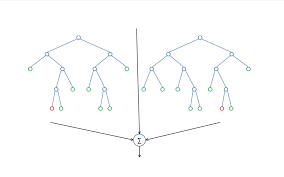
\includegraphics[scale=0.5]{figures/Chapter3AnnisaFathoroni1.png}
\caption{Random Forest}
\label{contoh}
\end{figure}

\end{itemize}

\item Cara Membaca Dataset

Berikut adalah cara membaca dataset :
\begin{itemize}
\item Buka Anaconda Navigator lalu jalankan Syder, kemudian import libraries yang dibutuhkan.
\item Masukkan kode python untuk membaca file csv, lalu jalankan

\begin{figure}[ht]
\centering
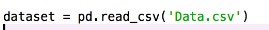
\includegraphics[scale=0.8]{figures/Chapter3AnnisaFathoroni5.jpeg}
\caption{Code Python}
\label{contoh}
\end{figure}

\item Maka pada window console akan menampilkan pesan berikut:

\begin{figure}[ht]
\centering

\includegraphics[scale=0.8]{figures/Chapter3AnnisaFathoroni6.jpeg}
\caption{Output}
\label{contoh}
\end{figure}

\item Dari explorer dapat terlihat dataset yang terimport.

\begin{figure}[ht]
\centering
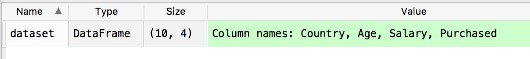
\includegraphics[scale=0.5]{figures/Chapter3AnnisaFathoroni7.jpeg}
\caption{Import Dataset}
\label{contoh}
\end{figure}

\item Lalu klik dataset cell, maka akan muncul seperti berikut :
\item Seperti yang terlihat pada gambar tersebut dataset ini memiliki Kolom Country, Age, dan Salary sebagai independent variable-nya dan kolom

\begin{figure}[ht]
\centering
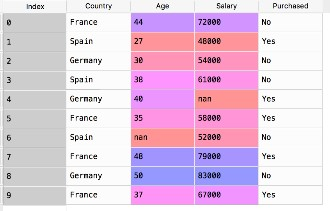
\includegraphics[scale=0.5]{figures/Chapter3AnnisaFathoroni8.jpeg}
\caption{Hasil Dataset Sel}
\label{contoh}
\end{figure}

\item Purchased sebagai dependent variable-nya.
\item Selanjutnya buat 2 matrix of features yang berisi values dari independent variable dan dependent variable.
\item Lalu tuliskan perintah berikut :

\begin{figure}[ht]
\centering

\includegraphics[scale=0.8]{figures/Chapter3AnnisaFathoroni9.jpeg}
\caption{Perintah}
\label{contoh}
\end{figure}

\item Perintah yang telah dibuat di atas akan membuat sebuah global environment baru dan muncul dataset.
\item Klik dataset tersebut maka muncul tabel berisi dataset.
\end{itemize}

\item Cross Validation

Cross-validation (CV) adalah metode statistik yang dapat digunakan untuk mengevaluasi kinerja model atau algoritma dimana data dipisahkan menjadi dua subset yaitu data proses pembelajaran dan data validasi / evaluasi. Model atau algoritma dilatih oleh subset pembelajaran dan divalidasi oleh subset validasi. Selanjutnya pemilihan jenis CV dapat didasarkan pada ukuran dataset. Biasanya CV K-fold digunakan karena dapat mengurangi waktu komputasi dengan tetap menjaga keakuratan estimasi.

\item Arti score 44\% pada random forest, 27\% pada decission tree dan 29\%dari SVM.

 Kalau maksud arti score 27\% pada decission tree adalah presentasi hasil dari perhitungan dataset, sedangkan maksud arti score 29\% dari SVM adalah hasil pendekatan jaringan saraf.  Hasil tersebut didapat dari hasil valdasi silang untuk memastikan bahwa membagi training test dengan cara yang berbeda. Sehingga didapat outputnya 44\% untuk hutan acak, 27\% untuk pohon keputusan, dan 29\% untuk SVM.

\item Confusion Matrix Dan Ilustrasinya
\begin{enumerate}
\item Perhitungan confusion matrix adalah sebagai berikut, akan saya beri contoh sederhana yaitu pengambilan keputusan untuk mendapatkan bantuan beasiswa. Saya menggunakan dua atribut, yaitu rekening listrik dan gaji. Ini adalah pohon keputusannya:
 
\begin{figure}[ht]
\centering
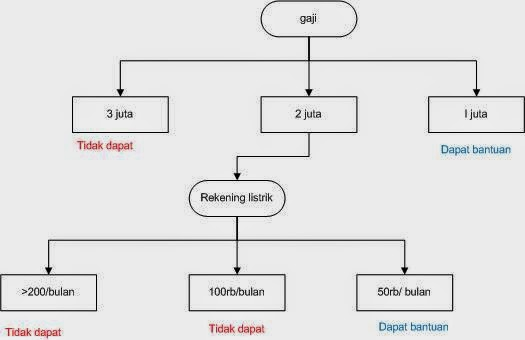
\includegraphics[scale=0.5]{figures/Chapter3AnnisaFathoroni2.jpg}
\caption{Pohon Keputusan}
\label{contoh}
\end{figure}
\end{enumerate}

Kemudian data testingnya adalah

\begin{figure}[ht]
\centering
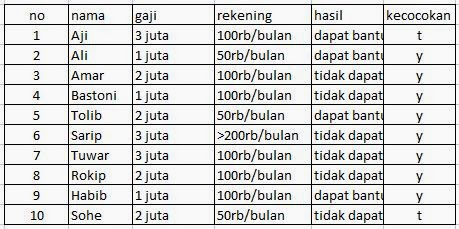
\includegraphics[scale=0.5]{figures/Chapter3AnnisaFathoroni3.jpg}
\caption{Data Testing}
\label{contoh}
\end{figure}

Yang pertama kita lakukan yaitu mencari 4 nilai yaitu a,b,c, dan d:

a= 5

b= 1

c= 1

d= 3

Kemudian kita dapat mencari nilai Recall, Precision, accuracy dan Error Rate

Recall =3/(1+3) = 0,75

Precision = 3/(1+3) = 0,75

Accuracy =(5+3)/(5+1+1+3) = 0,8

Error Rate =(1+1)/(5+1+1+3) = 0,2

\item Voting Random Forest Dan Ilustrasi Gambarnya.

\begin{itemize}
\item Pengertian Voting pada Random Forest

Metode ensemble dapat mencapai akurasi tinggi dengan membangun beberapa pengklasifikasi dan menjalankan masing-masing secara mandiri. Ketika classifier membuat keputusan, Anda dapat memanfaatkan yang terbaik keputusan umum dan rata-rata. Jika kita menggunakan metode yang paling umum, itu disebut voting

\item Ilustrasi Gambar Voting Random Forest :
\begin{figure}[ht]
\centering
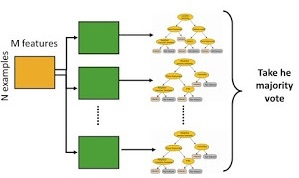
\includegraphics[scale=0.8]{figures/Chapter3AnnisaFathoroni4.jpg}
\caption{Voting Random Forest}
\label{contoh}
\end{figure}
\end{itemize}
\end{enumerate}
\chapter{Experiment and Result}
brief of experiment and result. Chapter 4

\section{Teori}
\section{Tasya Wiendhyra/1164086}
Hari Pertama Minggu Keempat
\subsection{Klasifikasi Teks}
\subsubsection{Pengertian Dan Ilustrasi}
Merupakan salah satu tugas terpenting dalam Pemrosesan Bahasa Alami (Natural Language Processing). Ini adalah proses mengklasifikasikan string teks atau dokumen ke dalam kategori yang berbeda, tergantung pada konten string. Klasifikasi teks memiliki berbagai aplikasi, seperti mendeteksi sentimen pengguna dari tweet, mengklasifikasikan email sebagai spam atau ham, mengklasifikasikan posting blog ke dalam kategori yang berbeda, penandaan otomatis permintaan pelanggan, dan sebagainya. BErikut adalah contoh dari Klasifikasi Teks.\\
Contohnya, misal kita ingin mencari kata dog, table, on, the . kemudian jika kata yang dimaksud sesuai maka akan menampilkan bilangan biner 1 dan jika salah 0. Seperti dibawah ini :
\begin{figure}[ht]
\centering
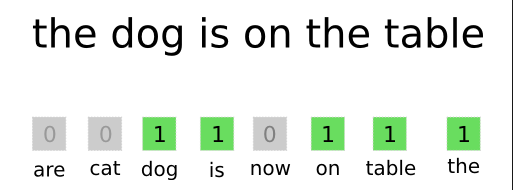
\includegraphics[scale=0.5]{figures/chapter4tasya1.png}
\caption{Klasifikasi Teks Tasya}
\label{Contoh}
\end{figure}
\\
\\
\\
\\
\subsection{Klasifikasi Bunga}
Jelaskan mengapa klasifikasi bunga tidak bisa menggunakan machine learning, sertakan ilustrasi sendiri.\\
Dikarenakan tidak semua bunga memliki ciri - ciri yang sama. Atau dalam kata lain terdapat data noise dalam klasifikasi bunga sehingga tidak bisa menggunakan machine learning.\\
Contohnya Anggrek memiliki warna ungu, dengan jumlah kelopak 5. Kemudian ada bunga warna ungu dengan jumlah kelopak yang sama namun ternyata bukan anggrek dan kategorinya banyak sekali. Bahkan ada bunga yang tidak jelas apakah warnanya sesuai atau tidak, sehingga bisa menyebabkan data noise.
\begin{figure}[ht]
\centering
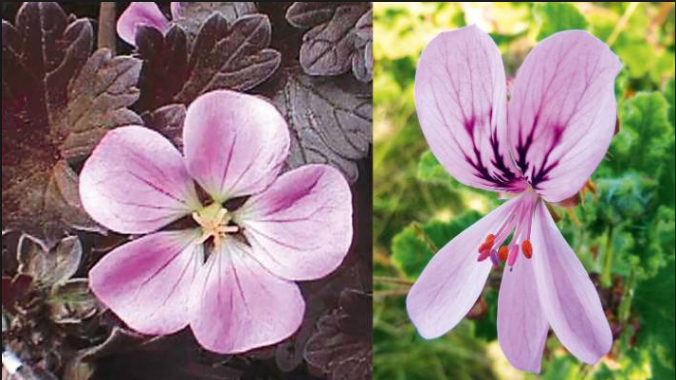
\includegraphics[scale=0.5]{figures/chapter4tasya2.png}
\caption{Klasifikasi Bunga Berwana Ungu Tasya}
\label{Contoh}
\end{figure}

\subsection{Pembelajaran Mesin Pada Teks Kata - Kata di Youtube}
Menggunakan teknik bag-of-words pada klasifikasi berbasis text dan kata untuk mengklasifikasikan komentar yang ada di internet sebagai spam atau bukan. Misalkan pada kolom komentar dapat di cek seberapa sering suatu kata muncul dalam kalimat. Setiap kata dapat dijadikan baris dan kolomnya ini merupakan kategori kata terbut, apakah masuk kedalam spam atau tidak. dan contoh lainnya yaitu pada Caption. dimana akan muncul subtitle secara otomatis dari youtube menggunakan sensor suara yang disesuaikan dengan kata yang telah ditentukan. Contohnya seperti berikut :
\begin{figure}[ht]
\centering
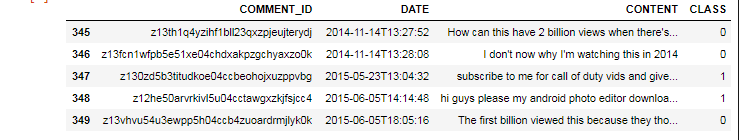
\includegraphics[scale=0.5]{figures/chapter4tasya3.png}
\caption{Klasifikasi Comment Spam Di Youtube Tasya}
\label{Contoh}
\end{figure}

\subsection{Arti Score 44\% Pada Random Forest, 27\% Pada Decission Tree Dan 29\% Dari SVM}
Itu merupakan presentase keakurasian prediksi yang dilakukan pada saat testing menggunakan label pada dataset yang digunakan. Score merupakan mendefinisikan aturan evaluasi model. Maka pada saat dijalankan akan muncuk persentase tersebut yang menunjukan keakurasian atau keberhasilan dari prediksi yang dilakukan. Jika menggunakan Random Forest maka hasilnya 40\% , jika menggunakan Decission Tree hasil prediksinya yaitu 27\% dan pada SVM 29\% .

\subsection{Bag of Words}
\subsubsection{Pengertian Dan Ilustrasi}
Merupakan representasi teks yang menggambarkan kemunculan kata-kata dalam dokumen. ePngelompokan kata kata kedalam perhitunga, berapakali sebuah kata muncul dalam satu kalimat. Disebut "tas" kata-kata, karena informasi tentang susunan atau struktur kata dalam dokumen dibuang. Model ini hanya berkaitan dengan apakah kata-kata yang diketahui muncul dalam dokumen, bukan di mana dalam dokumen.\\
Contohnya disini akan melihat kemunculan kata dari kalimat :
\begin{enumerate}
\item I Love Dogs
\item I hate dogs and knitting
\item Knitting is my hobby and passion. 
\end{enumerate}
\begin{figure}[ht]
\centering
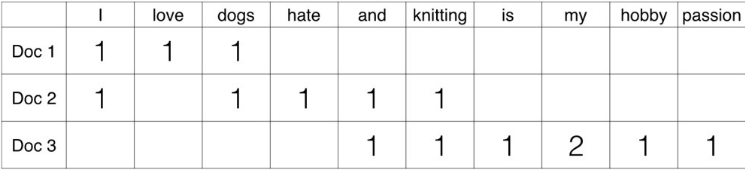
\includegraphics[scale=0.5]{figures/chapter4tasya4.png}
\caption{Bag of Words Tasya}
\label{Contoh}
\end{figure}

\subsection{TF-IDF}
\subsubsection{Pengertian Dan Ilustrasi}
TF-IDF  memberi kita frekuensi kata dalam setiap dokumen dalam korpus atau mengganti data jadi number. Ini adalah rasio berapa kali kata itu muncul dalam dokumen dibandingkan dengan jumlah total kata dalam dokumen itu. Itu meningkat seiring jumlah kemunculan kata itu di dalam dokumen meningkat. Setiap dokumen memiliki tf sendiri. Dalam ilustrasi disini saya akan mengganti contoh Bag of Words menjadi bentuk TF-IDF.
\begin{figure}[ht]
\centering
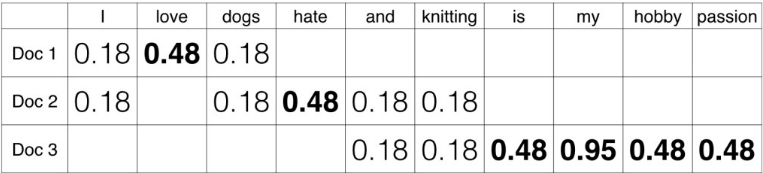
\includegraphics[scale=0.5]{figures/chapter4tasya5.png}
\caption{Contoh TF-IDF Tasya}
\label{Contoh}
\end{figure}
\chapter{Conclusion}
brief of conclusion

\section{Annisa Fathoroni/1164067}
\subsection{Teori}
Penjelasan Tugas Harian 9 ( No 1-6 )
\begin{enumerate}
\item Mengapa Kata-Kata Harus Di Lakukan Vektorisasi Dan Ilustrasi Gambar.
\begin{itemize}
\item Penjelasan:

Karenakan mesin hanya mampu membaca data dengan bentuk angka.Berdasarkan hal tersebut maka tentunya diperlukan vektorisasi kata atau bisa disebut dengan mengubah kata menjadi bentuk vektor agar mesin seolah-olah paham apa yang kita maksudkan dan dapat memproses aktifitas/perintah dengan benar. Selain alasan diatas, kata harus di vektorisasiuntuk mengetahui presentase kata yang sering muncul dalam setiap kalimatnya, yang berguna untuk menetukan kata kunci.

\item Ilustrasi Gambar

\begin{figure}[!hbtp]
\centering
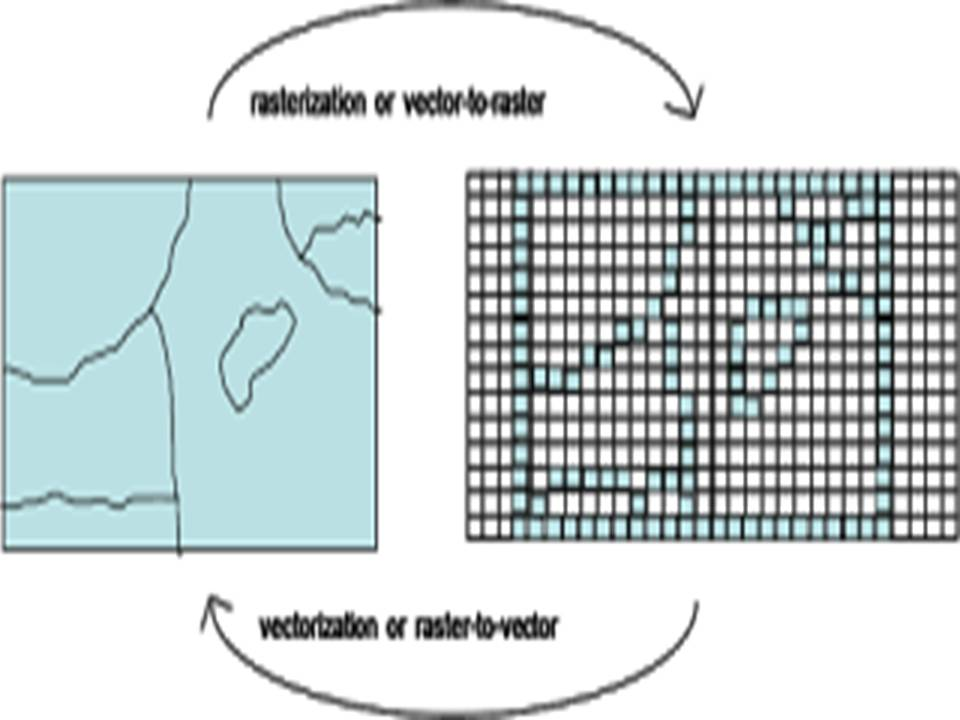
\includegraphics[scale=0.3]{figures/Chapter5AnnisaFathoroni5.jpg}
\caption{Vektorisasi - Annisa Fathoroni}
\label{Vektorisasi - Annisa Fathoroni}
\end{figure}

\end{itemize}

\item Mengapa Dimensi Dari Vektor Dataset Google Bisa Mencapai 300 Dan Ilustrasi Gambar.
\begin{itemize}
\item Penjelasan:

Karena pada masing-masing objek yang terdapat pada dataset akan memiliki identitasnya tersendiri. Apabila dicontohkan dengan penjelasan yang lebih rinci maka dilakukan perumpamaan sederhana. Misalnya untuk sebuah dataset google yang memiliki 3 buah objek yaitu berat, lebar, dan tinggi.  Kemudian dari masing-masing objek tersebut dilakukan perbandingan antara berat dan lebar beserta berat dan tinggi. Hasil yang didapatkan akan memiliki presentasi yang berbeda sehingga dapat diartikan bahwa mesin dapat membedakan objek yang hampir serupa namun tak sama.

\item Ilustrasi Gambar

\begin{figure}[!hbtp]
\centering
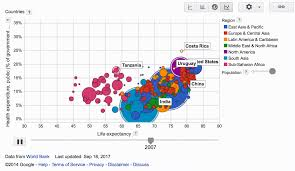
\includegraphics[scale=0.8]{figures/Chapter5AnnisaFathoroni7.jpg}
\caption{Dimensi Vektor Dataset - Annisa Fathoroni}
\label{Dimensi Vektor Dataset - Annisa Fathoroni}
\end{figure}

\end{itemize}

\item Konsep Vektorisasi Untuk Kata Dan Ilustrasi Gambar.
\begin{itemize}
\item  Penjelasan:

Konsep untuk vektorisasi kata sebenarnya sama dengan ketika dilakukan input suatu kata pada mesin pencarian. Kemudian untuk hasilnya akan mengeluarkan ( berupa ) referensi mengenai kata tersebut. Jadi data kata tersebut didapatkan dari hasil pengolahan pada kalimat-kalimat sebelumnya yang telah diolah. Contoh sederhananya pada kalimat berikut ( Please click the alarm icon for more notifications about my channel ), pada kalimat tersebut terdapat konteks yakni channel, kata tersebut akan dijadikan data latih untuk mesin yang akan dipelajari dan diproses. Jadi ketika kita inputkan kta channel, maka mesin akan menampilkan keterkaitannya dengan kata tersebut sehingga akan lebih efisien dan lebih mudah.

\item Ilustrasi Gambar

\begin{figure}[!hbtp]
\centering
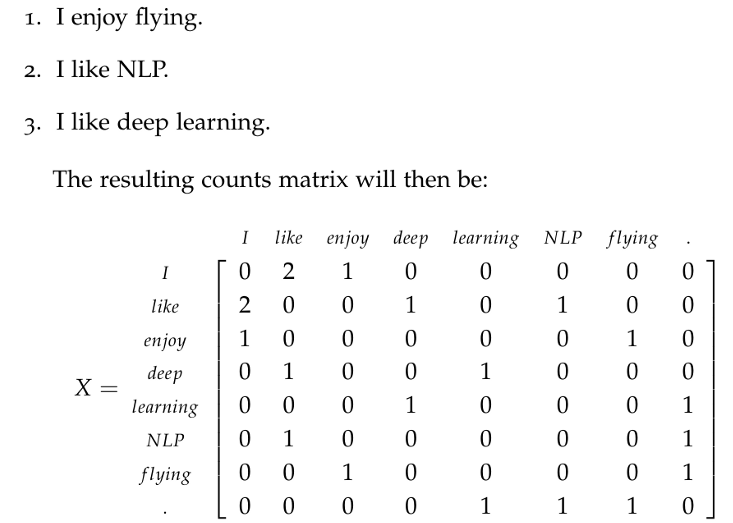
\includegraphics[scale=0.5]{figures/Chapter5AnnisaFathoroni4.png}
\caption{Vektorisasi Untuk Kata - Annisa Fathoroni}
\label{Vektorisasi Untuk Kata - Annisa Fathoroni}
\end{figure}

\end{itemize}

\item Konsep Vektorisasi Untuk Dokumen Dan Ilustrasi Gambar.
\begin{itemize}
\item  Penjelasan:

Untuk vektorisasi dokumen sebenarnya terbilang sama dengan konsep vektorisasi kata, yang membedakan hanya pada proses awalnya ( pada eksekusi awal ). Untuk vektorisasi dokumen ini, mesin akan membaca semua kalimat yang terdapat pada dokumen tersebut, kemudian kalimat yang terdapat pada dokumen tersebut akan di pecah menjadi kata-kata. Seperti itulah konsep vektorisasi dokumen.

\item Ilustrasi Gambar

\begin{figure}[!hbtp]
\centering
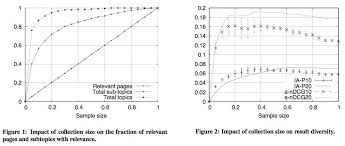
\includegraphics[scale=0.8]{figures/Chapter5AnnisaFathoroni6.jpg}
\caption{Vektorisasi Untuk Dokumen - Annisa Fathoroni}
\label{Vektorisasi Untuk Dokumen - Annisa Fathoroni}
\end{figure}

\end{itemize}

\item Pengertian Mean Dan Standar Devisiasi Beserta Ilustrasi Gambar.
\begin{itemize}
\item  Pengertian Mean:

Mean adalah nilai rata-rata dari beberapa buah data. Nilai mean dapat ditentukan dengan membagi jumlah data dengan banyaknya data. Mean (rata-rata) merupakan suatu ukuran pemusatan data. Mean suatu data juga merupakan statistik karena mampu menggambarkan bahwa data tersebut berada pada kisaran mean data tersebut. Mean tidak dapat digunakan sebagai ukuran pemusatan untuk jenis data nominal dan ordinal.

\item  Pengertian Standar Devisiasi:

Standar Deviasi dan Varians Salah satu teknik statistik yg digunakan untuk menjelaskan homogenitas kelompok. Varians merupakan jumlah kuadrat semua deviasi nilai-nilai individual thd rata-rata kelompok. Sedangkan akar dari varians disebut dengan standar deviasi atau simpangan baku. Standar Deviasi dan Varians Simpangan baku merupakan variasi sebaran data. Semakin kecil nilai sebarannya berarti variasi nilai data makin sama Jika sebarannya bernilai 0, maka nilai semua datanya adalah sama. Semakin besar nilai sebarannya berarti data semakin bervariasi.

\item Ilustrasi Gambar

\begin{figure}[!hbtp]
\centering
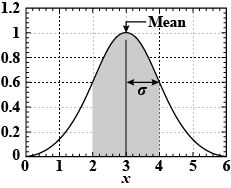
\includegraphics[scale=0.7]{figures/Chapter5AnnisaFathoroni2.png}
\caption{Mean - Annisa Fathoroni}
\label{Mean - Annisa Fathoroni}
\end{figure}

\begin{figure}[!hbtp]
\centering
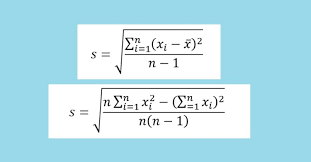
\includegraphics[scale=0.7]{figures/Chapter5AnnisaFathoroni3.png}
\caption{Standar Devisiasi - Annisa Fathoroni}
\label{Standar Devisiasi - Annisa Fathoroni}
\end{figure}

\end{itemize}

\item Penjelasan Skip-gram Dan Ilustrasi Gambar
\begin{itemize}
\item  Penjelasan:

Skip-Gram adalah kebalikannya, yaitu mencoba memprediksi vektor kata-kata yang ada di konteks diberikan vektor kata tertentu. Skip-Gram membuat sepasang kata target dan konteks sebagai sebuah instance sehingga Skip-Gram cenderung lebih baik ketika ukuran corpus sangat besar. 

\item Ilustrasi Gambar

\begin{figure}[!hbtp]
\centering
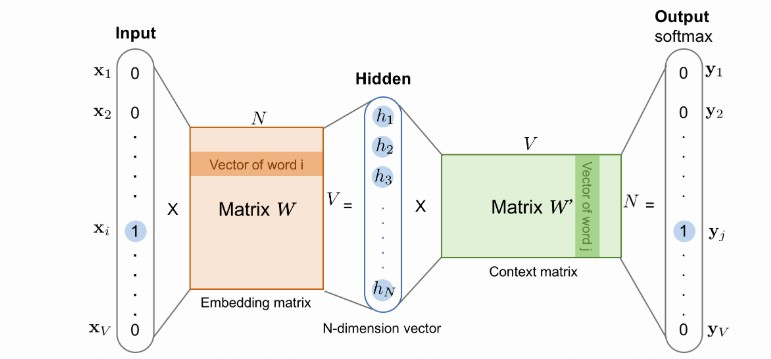
\includegraphics[scale=0.5]{figures/Chapter5AnnisaFathoroni1.jpg}
\caption{Skip Gram - Annisa Fathoroni}
\label{Skip Gram - Annisa Fathoroni}
\end{figure}
\par
\par
\end{itemize}
\par
\par
\end{enumerate}


\section{Tasya Wiendhyra /1164086}
HARI PERTAMA MINGGU KELIMA

\subsection{Kenapa Kata-Kata Harus Di Lakukan Vektorisasi Beserta Ilustrasi}
Karena ketika menggunakan algoritma machine learning tidak bisa  secara langsung menggunakan teks melainkan teks tersebut harus diubah menjadi angka. Kita membutuhkan cara untuk merepresentasikan data teks untuk algoritma pembelajaran mesin, vektorirasi membantu mengubah teks biasa kedalam bentuk vektor yang dapat dimengerti oleh komputer atau machine learning. Kita mungkin ingin melakukan klasifikasi dokumen, sehingga setiap dokumen adalah "input" dan label kelas adalah "output" untuk algoritma prediksinyai. Algoritma mengambil vektor angka sebagai input, oleh karena itu kita perlu mengkonversi dokumen menjadi vektor angka dengan panjang tetap atau sama.
\par Untuk ilustrasinya misal,  saya memiliki kamus berisikan kata-kata {MonkeyLearn, is, not, great}, dan saya ingin membuat vektor teks "MonkeyLearn is great", saya akan memiliki vektor berikut: (1, 1, 0, 0, 1,) .

\subsection{Mengapa Dimensi Dari Vektor Dataset Google Bisa Sampai 300 Beserta Ilustrasi}
Karena di dalam satu dataset berisikan setidaknya 3 Milyar kata dan kalimat. Yang dimana dimensi berisikan kata - kata unik dari data tersebut. Maka dari itu dimensi pada dataset Google bisa mencapai 300.

Untuk ilustrasinya, misalkan kita memiliki sebuah buku dengan tebal 1000 , dimana bukunya dibagi menjadi dua Chapter. Kemudian kita akan menggabungkan kata dari setiap Chapter tersebut. Maka akan didapatkan irisan yang akan berjumlah lebih dari 200. dikarenakan banyak kata yang berbeda beda.

\subsection{Konsep Vektorisasi Untuk Kata}
Konsepnya yaitu kata atau teks akan dihapuskan noisy datanya atau dihapus data yang tidak terpakai, seperti tag html jika ada, titik, koma, dll. Kemudian tokenization artinya kita akan mengelompokan kalimat menjadi token atua membagi kata kata menjadi potingan kecil. Baru setelah itu dilakukan normalisasi untuk mengubah datanya menjadi angka.

Ilustrasinya, misalnya ada beberapa kalimat seperti berikut :
\begin{itemize}
\item There used to be Iron Age.

Kemudian didapatkan token seperti berikut “There”,”was”,”to”,”be”,”used”,”Stone”,”Bronze,”Iron”,”Revolution”,”Digital”,”Age”,”of”,”Now”,”it”,”is”

Maka ketika di cek pada kalimat diatas hasilya seperti berikut 
\item There used to be iron age = [1,0,1,1,1,0,0,1,0,0,1,0,0,0,0]
\end{itemize}

\subsection{Konsep Vektorisasi Untuk Dokumen}
Hampir mirip dengan konsep kata, namun untuk di dokumen biasanya konsepnya digunakan untuk mencari kesamaan atau memprediksi seberapa sering menculan kata dalam 2 kalimat atau 2 paragraf.

Ilustrasinya, misalkan dalam sebuah artikel kita ingin mencari seberapa banyak kata "dimana" muncul. Maka dengan Doc2Vec dapat diprediksi hasilnya.

\subsection{Mean Dan Standar Deviasi}
\subsubsection{Pengertian}
Mean adalah nilai rata-rata dari beberapa buah data. Nilai mean dapat ditentukan dengan membagi jumlah data dengan banyaknya data.

Deviasi standar adalah ukuran ringkasan perbedaan setiap pengamatan dari rata-rata. Deviasi standar mengukur penyebaran data tentang nilai rata-rata. Ini berguna dalam membandingkan set data yang mungkin memiliki mean yang sama tetapi rentang yang berbeda.

\subsubsection{Contoh}
\begin{enumerate}
\item Misalkan kita sudah menghitung tinggi anjing.
\begin{figure}[ht]
\centering
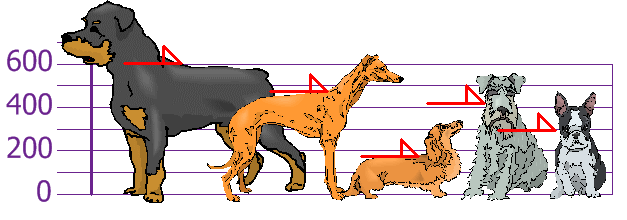
\includegraphics[scale=0.5]{figures/chapter5tasya1.png}
\caption{Contoh Mean dan Standar Deviasi }
\label{Teori}
\end{figure}
\item Tingginya dilihat dari bahu : 600mm, 470mm, 170mm, 430mm and 300mm.
\item Kita hitung mean atau rata ratanya, dengan menjumlahkan seluruh data dan membaginya dengan jumlah n nya hasilnya yaitu 394.
\item Kemudian kita ingin melihat berapa perbedaan tinggi dari anjing - anjing tersebut menggunakan variance. 
\item Baru Gunakan standar deviasi didapatkan hasil 147 mm . DEngan Deviasi Standar kita bisa tahau mana anjing dengan tinggi normal dan anjing yang kekurangan tinggi.
\begin{figure}[ht]
\centering
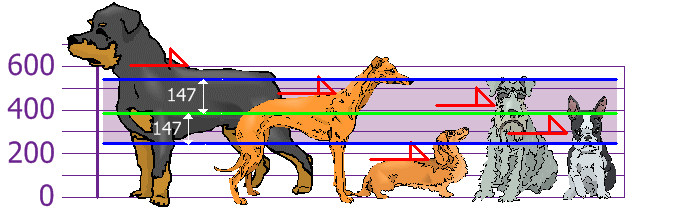
\includegraphics[scale=0.5]{figures/chapter5tasya2.png}
\caption{Contoh Mean dan Standar Deviasi }
\label{Teori}
\end{figure}

\subsection{Skip-gram}
Arsitektur model Skip-gram biasanya  mencoba untuk memprediksi kata konteks sumber (kata-kata sekitarnya) diberi kata target (kata tengah). Contohnya seperti berikut 
\begin{figure}[ht]
\centering
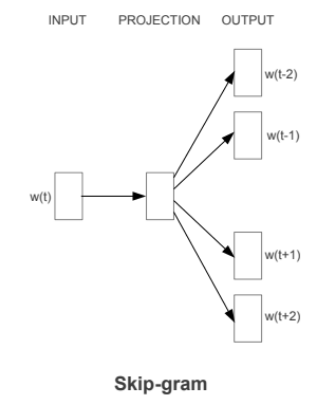
\includegraphics[scale=0.5]{figures/chapter5tasya3.png}
\caption{Contoh Skipgram }
\label{Teori}
\end{figure}
\end{enumerate}


\section{Annisa Cahyani-1164066}
\subsection{Teori}
Penjelasan Tugas Harian 9 ( No 1-6 ). 
\begin{enumerate}
\item Mengapa Kata Harus Di Lakukan Vektorisasi Dan Ilustrasi Gambar
\begin{itemize}
\item Mengapa kata ini harus dilakukan vektorisasi terlebih dahulu karena mesin tersebut hanya mampu atau dapat  membaca data yang berupa angka. Sehingga diperlukannya suatu  vektorisasi kata atau yang bisa disebut dengan mengubah suatu kata menjadi bentuk vektor agar mesin seolah paham apa yang telah kita maksud dan dapat memproses aktifitas atau perintah dengan betul.
\par
\end{itemize}
\par
\par
\item Mengapa Dimensi Dari Vektor Dataset Google Bisa Mencapai 300 Dan Ilustrasi Serta Contoh Gambar
\begin{itemize}
\item Konsep vektorisasi untuk kata yaitu sebuah dimensi dari suatu Vektor Dataset Google yang dapat mencapai 300  dikarenakan pada masing-masing objek yang telah terdapat pada dataset maka akan memiliki suatu identitasnya tersendiri.
\par
\end{itemize}
\par
\par
\item Konsep Vektorisasi Untuk Kata Dan Ilustrasi Gambar
\begin{itemize}
\item Penjelasan tetang vektorisasi untuk kata
\par Vektorisasi Kata adalah suatu hal yang sama dengan pada saat  kita menginputkan suatu kata pada mesin pencari. Kemudian akan  mengeluarkan hasil yang berupa suatu referensi mengenai kata tersebut. Sehingga hasil dari data kata tersebut akan didapatkan dari hasil pengolahan pada kalimat yang telah diolah sebelumnya.
\end{itemize}
\par
\par
\item Konsep Vektorisasi Untuk Dokumen Dan Ilustrasi Gambar
\begin{itemize}
\item Penjelasan tentang vektorisasi untuk dokumen
\par Vektorisasi dokumen yaitu suatu data yang terstruktur karena jauh dari bentuk table baris dan kolom, sehingga Perlu pembentukan data yang terstruktur untuk mewakili dokumen. Maka dari itu kita harus menentukan features yang mewakiliki seluruh kumpulan dokumen.
\end{itemize}
\par
\par
\item Pengertian Mean Dan Standar Devisiasi Beserta Ilustrasi Gambar
\begin{itemize}
\item Penjelasan Mean :
\par Mean yaitu  merupakan suatu nilai rata-rata dari suatu data. Sedangkan mean sendiri juga  dapat dicari dengan menggunakan cara membagi jumlah data dengan banyaknya data, maka dar itulah diperoleh  nilai rata-rata dari suatu data yang dicari.
\par
\item Penjelasan Standar Devisiasi :
\par standar deviasi merupakan sebuah teknik statistik yang diaman digunakan untuk menjelaskan homogenitas kelompok ataupun yang dapat diartikan sebagai nilai statistic. Yang  dimanfaatkan untuk menentukan bagaimana sebaran data pada dalam sampel, serta seberapa dekat dengan  titik data individu ke mean atau  ke rata-rata nilai sampel yang telah ada.
\par
\end{itemize}
\par
\par
\item Penjelasan Skip-gram Dan Ilustrasi Gambar
\begin{itemize}
\item Penjelasan skip-gram
\par Skip-Gram adalah dibutuhkan setiap kata yang ada dalam fokus dan juga mengambil satu-per-satu kata yang ditentukan untuk diberikan setelah pelatihan akan memprediksi probabilitas untuk setiap kata untuk benar-benar muncul di jendela di sekitar kata fokus.
\par
\par
\end{itemize}
\par
\par
\par
\par
\end{enumerate}


\section{PRAKTEK PROGRAM}
\section{Tasya Wiendhyra/1164086}
Praktek Hari Kedua Minggu Kelima
\subsection{Mencoba Dataset}
\subsubsection{Vektor}
\begin{itemize}
\item Pada gambar diatas dapat dilihat bahwa vektor memiliki array sebanyak 300 dimensi. Untuk identitas sektor satu adalah 0.10
\begin{figure}[ht]
\centering
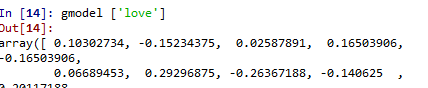
\includegraphics[scale=0.5]{figures/chapter5tasya4.png}
\caption{Vektor Love Tasya}
\label{Praktek}
\end{figure}


\item Pada gambar diatas untuk vektor faith dapat dilihat memliki nilai 0.26 , untuk similaritasnya cukup mendekati vektor love dimana faith dapat dikategorikan dalam satu kategori dengan love.
\begin{figure}[ht]
\centering
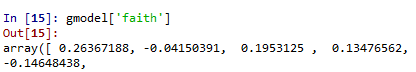
\includegraphics[scale=0.5]{figures/chapter5tasya5.png}
\caption{Vektor Faith Tasya}
\label{Praktek}
\end{figure}


\item Vektor fall hanya memiliki nilai minus yaitu -0.04 , dimana mesin memahami bahwa fall tidak terdapat dalam satu kategori yang sama dengan love dan faith
\begin{figure}[ht]
\centering
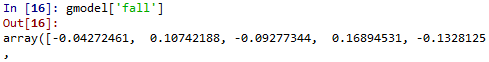
\includegraphics[scale=0.5]{figures/chapter5tasya6.png}
\caption{Vektor Fall Tasya}
\label{Praktek}
\end{figure}


\item  Vektor sick memiliki nilai identitas 1.82 dimana tidak mendekati love, faith maupun fall.
\begin{figure}[ht]
\centering
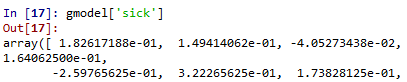
\includegraphics[scale=0.5]{figures/chapter5tasya7.png}
\caption{Vektor Sick Tasya}
\label{Praktek}
\end{figure}


\item Vektor clear memiliki nilai identitas -2,44 dan tidak mendekati nilai dari vektor fall sehingga tidak dapat dijadikan dalam satu kategori
\begin{figure}[ht]
\centering
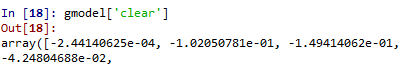
\includegraphics[scale=0.3]{figures/chapter5tasya8.png}
\caption{Vektor Clear Tasya}
\label{Praktek}
\end{figure}

\item Untuk vektor shine -0.12 tidak mendekati vektor manapun.
\begin{figure}[ht]
\centering
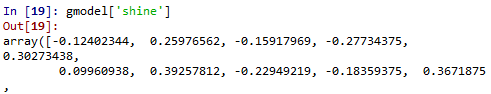
\includegraphics[scale=0.3]{figures/chapter5tasya9.png}
\caption{Vektor Shine Tasya}
\label{Praktek}
\end{figure}


\item Vektor bag memiliki i=nilai identitas -0.03 yang mendekati dengan vektor fall. SEhingga mesin memahami bahwa mungkin saja kedua vektor tersebut berada dalam satu kategori.
\begin{figure}[ht]
\centering
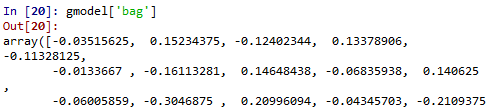
\includegraphics[scale=0.3]{figures/chapter5tasya10.png}
\caption{Vektor Bag Tasya}
\label{Praktek}
\end{figure}


\item Vektor car nilainya 0.13 mendekati vektor love dan faith sehingga mungkin dapat dikategorikan dalam satu kategori.
\begin{figure}[ht]
\centering
\includegraphics[scale=0.3]{figures/chapter5tasya11.png}
\caption{Vektor Car Tasya}
\label{Praktek}
\end{figure}


\item Vektor wash memiliki nilai 9.46 jauh dari vektor vektor lainnya.
\begin{figure}[ht]
\centering
\includegraphics[scale=0.3]{figures/chapter5tasya12.png}
\caption{Vektor Wash Tasya}
\label{Praktek}
\end{figure}


\item Vektor motor memiliki nilai identitas 5.73 yang bisa mendekati vektor wash. Dapat dikatakan bahwa motor dapat dicuci jika diarti dalam satu kategori yang sama.
\begin{figure}[ht]
\centering
\includegraphics[scale=0.3]{figures/chapter5tasya13.png}
\caption{Vektor Motor Tasya}
\label{Praktek}
\end{figure}
\end{itemize}

\subsubsection{Similariti}
\begin{enumerate}
\item Lihat gambar berikut yang merupakan hasil prediksi similariti
\begin{figure}[ht]
\centering
\includegraphics[scale=0.3]{figures/chapter5tasya17.png}
\caption{Similariti Tasya}
\label{Praktek}
\end{figure}

Dapat disimpulkan bahwa
\begin{itemize}
\item Untuk Love dan faith hasilnya adalah 37%
\item Untuk Love dan fall hasilnya adalah 11%
\item Untuk Love dan sick hasilnya adalah 26%
\item Untuk Love dan clear hasilnya adalah 6%
\item Untuk Love dan shine hasilnya adalah 20%
\item Artinya love dan faith memang dalam kategoruiyang sama misalnya dalam kategori percintaan. MEsin sudah mengetahui bahwa keduanya dapat dikategorikan sebagai percintaan.
\end{itemize}
\end{enumerate}

\subsection{Extract Words dan PermuteSentences}
\subsubsection{Extract Words}
ExtractWords merupakan function untuk menambahkan, menghilangkan atau menghapuskan, hal hal yang tidak penting atau tidakperlu di dalam teks. Dalam contoh dibawah ini. menggunakan function extract words untuk menghapus komen dengan python style , mencari data yang diinginkan, dan memberikan spasi pada teks.
\begin{figure}[ht]
\centering
\includegraphics[scale=0.3]{figures/chapter5tasya15.png}
\caption{Extract Words Tasya}
\label{Praktek}
\end{figure}

\subsubsection{PermuteSentences}
PermuteSentences merupakan class yang digunakan unutm melakukan pengocokan secara acak pada data yang ada. Digunakan cara ini agar tidak terjadi kelebihan memori pada saat dijalankan. Contoh dibawah yaitu fungsi akan memanggil lenght. Yang kemudian mendefinisikan variabel req untuk lenght dam melakukan random choice yaitu pengocokan acak untuk kata car.
\begin{figure}[ht]
\centering
\includegraphics[scale=0.3]{figures/chapter5tasya16.png}
\caption{PermuteSentencesi Tasya}
\label{Praktek}
\end{figure}

\section{Annisa Fathoroni/1164067}
\subsection{Praktek}
Penjelasan Tugas Harian 10 ( No 1-10 ). ( Dan Penanganan Error )
\begin{enumerate}
\item Percobaan Google Dataset ( Perbandingan Dan Similarity ) Untuk Beberapa Data Berikut :
\begin{enumerate}
\item Love

Penjelasan: Pada hasil gambar 'love' dapat dilihat bahwa nilai pada vektor baris pertamanya adalah 0.10302734. Jika dibandingkan dengan gambar 'faith' dapat dikatakan bahwa kedua gambar tersebut tidak dapat dimasukkan pada kategori yang sama.

\begin{figure}[!hbtp]
\centering
\includegraphics[scale=0.7]{figures/Chapter5AnnisaFathoroni12love.jpg}
\caption{Google Dataset - Annisa Fathoroni, love.}
\label{Google Dataset - Annisa Fathoroni, love.}
\end{figure}

\item Faith

Penjelasan: Pada hasil gambar 'faith' dapat dilihat bahwa nilai pada vektor baris pertamanya adalah 0.26367188. Jika dibandingkan dengan gambar 'fall' dapat dikatakan bahwa kedua gambar tersebut tidak dapat dimasukkan pada kategori yang sama.

\begin{figure}[!hbtp]
\centering
\includegraphics[scale=0.7]{figures/Chapter5AnnisaFathoroni13faith.jpg}
\caption{Google Dataset - Annisa Fathoroni, faith.}
\label{Google Dataset - Annisa Fathoroni, faith.}
\end{figure}

\item Fall

Penjelasan: Pada hasil gambar 'fall' dapat dilihat bahwa nilai pada vektor baris pertamanya adalah -0.04272461. Jika dibandingkan dengan gambar 'sick' dapat dikatakan bahwa kedua gambar tersebut tidak dapat dimasukkan pada kategori yang sama.

\begin{figure}[!hbtp]
\centering
\includegraphics[scale=0.7]{figures/Chapter5AnnisaFathoroni14fall.jpg}
\caption{Google Dataset - Annisa Fathoroni, fall.}
\label{Google Dataset - Annisa Fathoroni, fall.}
\end{figure}

\item Sick

Penjelasan: Pada hasil gambar 'sick' dapat dilihat bahwa nilai pada vektor baris pertamanya adalah 1.82617188e-01. Jika dibandingkan dengan gambar 'clear' dapat dikatakan bahwa kedua gambar tersebut tidak dapat dimasukkan pada kategori yang sama.

\begin{figure}[!hbtp]
\centering
\includegraphics[scale=0.7]{figures/Chapter5AnnisaFathoroni15sick.jpg}
\caption{Google Dataset - Annisa Fathoroni, sick.}
\label{Google Dataset - Annisa Fathoroni, sick.}
\end{figure}

\item Clear

Penjelasan: Pada hasil gambar 'clear' dapat dilihat bahwa nilai pada vektor baris pertamanya adalah -2.44140625e-04. Jika dibandingkan dengan gambar 'shine' dapat dikatakan bahwa kedua gambar tersebut tidak dapat dimasukkan pada kategori yang sama.

\begin{figure}[!hbtp]
\centering
\includegraphics[scale=0.7]{figures/Chapter5AnnisaFathoroni16clear.jpg}
\caption{Google Dataset - Annisa Fathoroni, clear.}
\label{Google Dataset - Annisa Fathoroni, clear.}
\end{figure}

\item Shine

Penjelasan: Pada hasil gambar 'shine' dapat dilihat bahwa nilai pada vektor baris pertamanya adalah -0.12402344. Jika dibandingkan dengan gambar 'bag' dapat dikatakan bahwa kedua gambar tersebut tidak dapat dimasukkan pada kategori yang sama.

\begin{figure}[!hbtp]
\centering
\includegraphics[scale=0.7]{figures/Chapter5AnnisaFathoroni17shine.jpg}
\caption{Google Dataset - Annisa Fathoroni, shine.}
\label{Google Dataset - Annisa Fathoroni, shine.}
\end{figure}

\item Bag

Penjelasan: Pada hasil gambar 'bag' dapat dilihat bahwa nilai pada vektor baris pertamanya adalah -0.03515625. Jika dibandingkan dengan gambar 'car' dapat dikatakan bahwa kedua gambar tersebut tidak dapat dimasukkan pada kategori yang sama.

\begin{figure}[!hbtp]
\centering
\includegraphics[scale=0.7]{figures/Chapter5AnnisaFathoroni18bag.jpg}
\caption{Google Dataset - Annisa Fathoroni, bag.}
\label{Google Dataset - Annisa Fathoroni, bag.}
\end{figure}

\item Car

Penjelasan: Pada hasil gambar 'car' dapat dilihat bahwa nilai pada vektor baris pertamanya adalah 0.13085938. Jika dibandingkan dengan gambar 'wash' dapat dikatakan bahwa kedua gambar tersebut tidak dapat dimasukkan pada kategori yang sama.

\begin{figure}[!hbtp]
\centering
\includegraphics[scale=0.7]{figures/Chapter5AnnisaFathoroni19car.jpg}
\caption{Google Dataset - Annisa Fathoroni, car.}
\label{Google Dataset - Annisa Fathoroni, car.}
\end{figure}

\item Wash

Penjelasan: Pada hasil gambar 'wash' dapat dilihat bahwa nilai pada vektor baris pertamanya adalah 9.46044922e-03. Jika dibandingkan dengan gambar 'motor' dapat dikatakan bahwa kedua gambar tersebut tidak dapat dimasukkan pada kategori yang sama.

\begin{figure}[!hbtp]
\centering
\includegraphics[scale=0.7]{figures/Chapter5AnnisaFathoroni20wash.jpg}
\caption{Google Dataset - Annisa Fathoroni, wash.}
\label{Google Dataset - Annisa Fathoroni, wash.}
\end{figure}

\item Motor

Penjelasan: Pada hasil gambar 'motor' dapat dilihat bahwa nilai pada vektor baris pertamanya adalah 5.73730469e-02. Jika dibandingkan dengan gambar 'cycle' dapat dikatakan bahwa kedua gambar tersebut tidak dapat dimasukkan pada kategori yang sama.

\begin{figure}[!hbtp]
\centering
\includegraphics[scale=0.7]{figures/Chapter5AnnisaFathoroni21motor.jpg}
\caption{Google Dataset - Annisa Fathoroni, motor.}
\label{Google Dataset - Annisa Fathoroni, motor.}
\end{figure}

\item Cycle

Penjelasan: Pada hasil gambar 'cycle' dapat dilihat bahwa nilai pada vektor baris pertamanya adalah 0.04541016. Jika dibandingkan dengan gambar 'love' dapat dikatakan bahwa kedua gambar tersebut tidak dapat dimasukkan pada kategori yang sama.

\begin{figure}[!hbtp]
\centering
\includegraphics[scale=0.7]{figures/Chapter5AnnisaFathoroni22cycle.jpg}
\caption{Google Dataset - Annisa Fathoroni, cycle.}
\label{Google Dataset - Annisa Fathoroni, cycle.}
\end{figure}

\item Similarity

Penjelasan: Pada hasil gambar 'car' dapat dilihat bahwa nilai pada vektor baris pertamanya adalah 0.13085938. Jika dibandingkan dengan gambar 'love', 'sick', 'clear', 'motor', 'wash' dapat dikatakan bahwa semua gambar tersebut yang paling mendekati adalah 'sick'.

\begin{figure}[!hbtp]
\centering
\includegraphics[scale=0.7]{figures/Chapter5AnnisaFathoroni23.jpg}
\caption{Google Dataset - Annisa Fathoroni, similarity.}
\label{Google Dataset - Annisa Fathoroni, similarity.}
\end{figure}

\end{enumerate}

\item Penjelasan Dan Ilustrasi ExtractWords Dan PermuteSentences
\begin{itemize}

\begin{figure}[!hbtp]
\centering
\includegraphics[scale=0.7]{figures/Chapter5AnnisaFathoroni32.jpg}
\caption{Extract Word dan PermuteSentences - Annisa Fathoroni}
\label{Extract Word dan PermuteSentences - Annisa Fathoroni}
\end{figure}

\item ExtractWords

Penjelasan:  Pada kalimat 'This isn't really a sentence' yang  akan dipisahkan perkata. Dimana library re dan library string di import terlebih dahulu. Lalu variable out mendefinisikan X untuk mengembalikan string pada objek line yang telah di split. Kemudian, X dikembalikan berdasarkan jumlah kata.

\begin{figure}[!hbtp]
\centering
\includegraphics[scale=0.7]{figures/Chapter5AnnisaFathoroni29.jpeg}
\caption{ExtractWord - Annisa Fathoroni}
\label{ExtractWord - Annisa Fathoroni}
\end{figure}

\item PermuteSentences

Penjelasan: Digunakan untuk melakukan pengocokan atau acak pada text yang diiginkan.

\begin{figure}[!hbtp]
\centering
\includegraphics[scale=0.7]{figures/Chapter5AnnisaFathoroni31.jpg}
\caption{PermuteSentences - Annisa Fathoroni}
\label{PermuteSentences - Annisa Fathoroni}
\end{figure}

\end{itemize}
\end{enumerate}
\chapter{Discussion}
Please tell more about conclusion and how to the next work of this study.

\section{Annisa Fathoroni/1164067}
\subsection{Teori}
Penjelasan Tugas Harian 11 ( No 1-8 ).
\begin{enumerate}
\item Mengapa file suara harus dilakukan MFCC, dilengkapi dengan ilustrasi atau gambar.

Mel Frequency Cepstral Coefficients (MFCC) merupakan koefisien yang merepresentasikan audio. Sehingga diharuskannya melakukan MFCC kepada objek suara atau audio agar suara dapat berubah atau diubah ke dalam bentuk data matrix dimana telah dilakukan ekstraksi oleh MFCC kemudian direalisasikan sebagai data matrix.

\begin{itemize}
\item Ilustrasi Gambar:

\begin{figure}[!hbtp]
\centering
\includegraphics[scale=0.7]{figures/Chapter6AnnisaFathoroni1.png}
\caption{MFCC - Annisa Fathoroni}
\label{MFCC - Annisa Fathoroni}
\end{figure}

\end{itemize}

\item Konsep dasar Neural Network, dilengkapi dengan ilustrasi atau gambar.

Neural Network merupakan replika dari sistem syaraf yang terdapat pada sistem otak manu- sia. Dalam proses kerjanya, otak manusia disusun atas miliaran neuron dimana masing-masing neuron akan terhubung pada puluhan ribu neuron lain.
\begin{itemize}
\item Ilustrasi Gambar:

\begin{figure}[!hbtp]
\centering
\includegraphics[scale=0.7]{figures/Chapter6AnnisaFathoroni2.jpg}
\caption{Konsep Dasar Neural Network - Annisa Fathoroni}
\label{Konsep Dasar Neural Network - Annisa Fathoroni}
\end{figure}

\end{itemize}

\item Konsep pembobotan Neural Network, dilengkapi dengan ilustrasi atau gambar.

Bobot merupakan suatu nilai yang mendefinisikan tingkat atau kepentingan hubungan antara suatu node dengan node yang lain. Semakin besar bobot  suatu hubungan menandakan semakin pentingnya hubungan kedua node tersebut. Bobot merupakan suatu hubungan berupa bilangan real maupun integer, tergantung dari jenis permasalahan dan model yang digunakan. Bobot-bobot tersebut bisa ditentukan untuk berada didalam interval tertentu. selama proses pelatihan, bobot tersebut dapat menyesuaikan dengan pola-pola input.

\begin{itemize}
\item Ilustrasi Gambar :

\begin{figure}[!hbtp]
\centering
\includegraphics[scale=0.7]{figures/Chapter6AnnisaFathoroni3.jpg}
\caption{Konsep Pembobotan Neural Network - Annisa Fathoroni}
\label{Konsep Pembobotan Neural Network - Annisa Fathoroni}
\end{figure}

\end{itemize}

\item Konsep fungsi aktifasi dalam Neural Network, dilengkapi dengan ilustrasi atau gambar.
Operasi matematik yang dikenakan pada sinyal output y. Sehingga fungsi ini akan digunakan untuk pengaktifan dan juga penonaktifan neuron.
\begin{itemize}
\item Dalam konsep fungsi aktivasi Neuron Network terdapat beberapa jenis:
\begin{itemize}
\item Fungsi Undak Biner Hard Limit ( Menkonversi nilai masukan dari suatu variabel )
\item Fungsi Undak Biner Threshold ( Menggunakan nilai ambang 0 sebagai batas eksekusil )
\item Fungsi Bipolar Symetric Hard Limit ( Mempunyai keluaran bernilai 1 dan 0 )
\item Fungsi Bipolar Threshold ( Mempunyai keluaran bernilai 1, 0 atau -1 )

\item Ilustrasi Gambar:

\begin{figure}[!hbtp]
\centering
\includegraphics[scale=0.7]{figures/Chapter6AnnisaFathoroni4.jpg}
\caption{Konsep Fungsi Aktifasi - Annisa Fathoroni}
\label{Konsep Fungsi Aktivasi - Annisa Fathoroni}
\end{figure}

\end{itemize}
\end{itemize}

\item Cara membaca hasil plot dari MFCC, dilengkapi dengan ilustrasi atau gambar.

Penjelasan Cara Membaca Hasil Plot Dari MFCC :
\begin{itemize}
\item Ilustrasi Gambar :
\begin{figure}[!hbtp]
\centering
\includegraphics[scale=0.4]{figures/Chapter6AnnisaFathoroni5.png}
\caption{Plot MFCC - Annisa Fathoroni}
\label{Plot MFCC - Annisa Fathoroni}
\end{figure}

\end{itemize}

\item Apa itu One-Hot Encoding, dilengkapi dengan ilustrasi atau gambar.


One-Hot Encoding adalah sekelompok bit yang kombinasi hukumnya hanya terdiri dari bit dengan bit tinggi (1) dan bit lainnya rendah (0). Implementasi serupa di mana semua bit '1' kecuali satu '0' kadang-kadang disebut one-cold. Dalam statistik, variabel dummy mewakili teknik serupa untuk mewakili data kategorikal.
\begin{itemize}
\item Ilustrasi Gambar:

\begin{figure}[!hbtp]
\centering
\includegraphics[scale=0.4]{figures/Chapter6AnnisaFathoroni6.png}
\caption{One-Hot Encoding - Annisa Fathoroni}
\label{One-Hot Encoding - Annisa Fathoroni}
\end{figure}

\end{itemize}

\item Fungsi dari np.unique dan to.categorical, dilengkapi dengan ilustrasi atau gambar.
\begin{enumerate}
\item np.unique:

Berfungsi untuk menemukan elemen unik array. Ada tiga output opsional selain elemen unik:

\begin{itemize}
\item Indeks array input yang memberikan nilai unik
\item Indeks array unik yang merekonstruksi array input
\item Berapa kali setiap nilai unik muncul dalam array input
\end{itemize}

\item Ilustrasi Gambar :

\begin{figure}[!hbtp]
\centering
\includegraphics[scale=0.7]{figures/Chapter6AnnisaFathoroni7-1.png}
\caption{np.unique - Annisa Fathoroni}
\label{np.unique - Annisa Fathoroni}
\end{figure}

\item to.categorical:

Berfungsi untuk mengubah vektor kelas yang berupa integer menjadi matriks kelas biner.

\begin{itemize}
\item Ilustrasi Gambar :

\begin{figure}[!hbtp]
\centering
\includegraphics[scale=0.7]{figures/Chapter6AnnisaFathoroni7-2.png}
\caption{to.categorical - Annisa Fathoroni}
\label{to.categorical - Annisa Fathoroni}
\end{figure}

\end{itemize}
\end{enumerate}

\item Fungsi dari Sequential, dilengkapi dengan ilustrasi atau gambar.
Sebuah jenis model yang digunakan dalam perhitungan ataupun code program yang direalisasikan.
\begin{itemize}
\item Ilustrasi Gambar:

\begin{figure}[!hbtp]
\centering
\includegraphics[scale=0.7]{figures/Chapter6AnnisaFathoroni8.png}
\caption{Sequential - Annisa Fathoroni}
\label{Sequential - Annisa Fathoroni}
\end{figure}

\end{itemize}
\end{enumerate}

\section{Tasya Wiendhyra / 1164086}
\subsection{Teori}
\begin{enumerate}
\item Kenapa file suara harus di lakukan MFCC. dilengkapi dengan ilustrasi atau gambar. \\
\par Nilai-nilai MFCC meniru pendengaran manusia dan mereka biasanya digunakan dalam aplikasi pengenalan suara serta genre musik
deteksi. Nilai-nilai MFCC ini akan dimasukkan langsung ke jaringan saraf.Agar dapat diubah menjadi bentuk vektor, dan dapat digunakan pada machine learning. Disebabkan machine learning hanya mengerti bilangan vektor saja.\\
Ilustrasinya, Ketika ingin menggunakan file suara dalam machine learning, misalnya untuk melihat jam. Machine learning tidak memahami rekaman suara melainkan vektor. Maka rekaman tersebut akan diubah kedalam bentuk vektor kemudian vektor akan menyesuaikan dengan kata kata yang sudah disediakan. Jika cocok maka akan mengembalikan waktu yang diinginkan

\item Konsep dasar neural network dilengkapi dengan ilustrasi atau gambar
\par Neural Network ini terinspirasi dari jaringan saraf otak manusia. Dimana setiap neuron terhubung ke setiap neuron di lapisan berikutnya. Lapisan pertama menerima input dan lapisan terakhir memberikan keluaran. Struktur jaringan, yang berarti jumlah neuron dan koneksinya, diputuskan sebelumnya dan tidak dapat berubah, setidaknya tidak selama training. Juga, setiap input harus memiliki jumlah nilai yang sama. Ini berarti bahwa gambar, misalnya, mungkin perlu diubah ukurannya agar sesuai dengan jumlah neuron input.\\

Ilustrasinya. misalkan kita ingin encode sebuah kalimat yaitu "what time is it" kemudian Anda menginisialisasi lapisan jaringan Anda dan hidden statel. Bentuk dan dimensi hidden state akan tergantung pada bentuk dan dimensi jaringan saraf berulang Anda. Kemudian Anda mengulangi input Anda, meneruskan kata danhidden state ke NN. NN mengembalikan output dan kondisi tersembunyi yang dimodifikasi. Anda terus mengulang sampai Anda kehabisan kata-kata. Terakhir Anda melewatkan output ke layer feedforward, dan itu mengembalikan prediksi. Bahwa kita ingin mengetahui pukul berapa sekarang.

\item Konsep pembobotan dalam neural network.dilengkapi dengan ilustrasi atau gambar
\par Bobot mewakili kekuatan koneksi antar unit. Jika bobot dari node 1 ke node 2 memiliki besaran lebih besar, itu berarti bahwa neuron 1 memiliki pengaruh lebih besar terhadap neuron. 2. Bobot penting untuk nilai input. Bobot mendekati nol berarti mengubah input ini tidak akan mengubah output. Bobot negatif berarti meningkatkan input ini akan mengurangi output. Bobot menentukan seberapa besar pengaruh input terhadap output. Seperti contoh berikut :
\begin{figure}[ht]
\centering
\includegraphics[scale=0.5]{figures/chapter6tasya2.png}
\caption{Contoh Pembobotan Neural Network Tasya}
\label{Teori}
\end{figure}

\item Konsep fungsi aktifasi dalam neural network. dilengkapi dengan ilustrasi atau gambar
\par Fungsi aktivasi digunakan untuk memperkenalkan non-linearitas ke jaringan saraf. Ini menekan nilai dalam rentang yang lebih kecil yaitu. fungsi aktivasi Sigmoid memeras nilai antara rentang 0 hingga 1. Ada banyak fungsi aktivasi yang digunakan dalam industri pembelajaran yang dalam dan ReLU, SeLU dan TanH lebih disukai daripada fungsi aktivasi sigmoid. Ilustrasinya, ketika fungsi aktivasi linier, jaringan saraf dua lapis mampu mendekati hampir semua fungsi. Namun, jika fungsi aktivasi identik dengan fungsi aktivasi F (X) = X), properti ini tidak puas, dan jika MLP menggunakan fungsi aktivasi yang sama, seluruh jaringan setara dengan jaringan saraf lapis tunggal.

\item Cara membaca hasil plot dari MFCC,dilengkapi dengan ilustrasi atau gambar\\
Berikut merupakan hasil plot dari rekaman suara :
\begin{figure}[ht]
\centering
\includegraphics[scale=0.5]{figures/chapter6tasya1.png}
\caption{Cara Membaca Hasil Plot MFCC Tasya}
\label{Teori}
\end{figure}
Dari gambar tersebut dapat diketahui :\\
\begin{itemize}
\item Terdapat 2 dimensi yaitu x sebagai waktu, dan y sebagai power atau desibel.
\item Dapat dilihat bahwa jika berwarna biru maka power dari suara tersebut rendah, dan jika merah power dari suara tersebut tinggi
\item Dibagian atas terdapat warna merah pudar yang menandakan bahwa tidak ada suara sama sekali dalam jangkauan tersebut.
\end{itemize}

\item Jelaskan apa itu one-hot encoding,dilengkapi dengan ilustrasi kode dan atau gambar.
\par One-hot encoding adalah representasi variabel kategorikal sebagai vektor biner. Mengharuskan nilai kategorikal dipetakan ke nilai integer. Kemudian, setiap nilai integer direpresentasikan sebagai vektor biner yang semuanya bernilai nol kecuali indeks integer, yang ditandai dengan 1.
\begin{figure}[ht]
\centering
\includegraphics[scale=0.5]{figures/chapter6tasya3.png}
\caption{One Hot Encoding Tasya}
\label{Teori}
\end{figure}

\item fungsi dari np/.unique dan to categorical dalam kode program,dilengkapi dengan ilustrasi atau gambar.\\
Untuk np unique fungsinya yaitu menemukan elemen unik array. Mengembalikan elemen unik array yang diurutkan. Ada tiga output opsional selain elemen unik:\\
\begin{itemize}
\item Indeks array input yang memberikan nilai unik
\item Indeks array unik yang merekonstruksi array input
\item Berapa kali setiap nilai unik muncul dalam array input.
\end{itemize}
\begin{figure}[ht]
\centering
\includegraphics[scale=0.5]{figures/chapter6tasya4.png}
\caption{Numpy Unique Tasya}
\label{Teori}
\end{figure}

Untuk  To Categorical fungsinya untuk mengubah vektor kelas (integer) ke matriks kelas biner.
\begin{figure}[ht]
\centering
\includegraphics[scale=0.5]{figures/chapter6tasya5.png}
\caption{To Categorical Tasya}
\label{Teori}
\end{figure}

\item Fungsi dari Sequential dalam kode program,dilengkapi dengan ilustrasi atau gambar.\\
Sequential berfungsi sebagai tumpukan linear lapisan. COntohnya sebagai berikut :
\begin{figure}[ht]
\centering
\includegraphics[scale=0.5]{figures/chapter6tasya6.png}
\caption{Sequential Tasya}
\label{Teori}
\end{figure}
\end{enumerate}

\section{Annisa Cahyani-1164066}
\subsection{Teori}
Penjelasan Tugas Harian11 ( No 1-8 )
\begin{enumerate}
\item Mengapa File Suara Harus Dilakukan MFCC Dilengkapi Dengan Ilustrasi Atau Gambar :
\par Yang Perlu kita ketahui disini yaitu  bahwa MFCC adalah Mel Frequency Cepstral Coefficients itu yang merupakan suatu koefisien yang merepresentasikan sebuah audio yang lebih simpel digunakan untuk sebagai library. 
\begin{itemize}
\item Penjelasan Mengenai  File Suara Harus Dilakukan MFCC : 
\par Yang harus kita ketahui itu pada saat ingin melakukan MFCC ini kepada sebuah objek suara agar suara itu tersebut dapat berubah atau dapat diubah ke dalam bentuk data matrix yang telah diekstraksi oleh MFCC.
\end{itemize}
\par
\par
\item Konsep Dasar Neural Network Dilengkapi Dengan Ilustrasi Atau Gambar :
\par Neural Network adalah paradigma pemrosesan suatu informasi yang terinspirasi oleh sistim sel syaraf biologi, sama seperti otak yang memproses suatu informasi. 
\begin{itemize}
\item Penjelasan Konsep Dasar Neural Network
\par Neural Network merupakan kategori ilmu Soft Computing. Neural Network sebenarnya mengadopsi dari kemampuan otak manusia yang mampu memberikan stimulasi atau rangsangan, melakukan proses, dan memberikan output. Output diperoleh dari variasi stimulasi dan proses yang terjadi di dalam otak manusia.
\par
\par
\item Konsep Fungsi Aktifasi Dalam Neural Network Dilengkapi Dengan Ilustrasi Atau Gambar :
\begin{itemize}
\item Penjelasan Konsep Fungsi Aktifasi Dalam Neural Network :
\par Operasi matematik yang dikenakan pada sinyal outputnya. Fungsi aktivasi, ini berfungsi untuk seperti sinapsis. 
\item Dalam Konsep Fungsi Aktivasi Neuron Network Terdapat Beberapa Jenis, Yaitu :
\begin{itemize}
\item Fungsi Undak Biner Hard Limit ini untuk menkonversi sebuah nilai masukan dari suatu variabel
\item Fungsi Undak Biner Threshold disini untuk menggunakan nilai yang ambang 0 untuk batas eksekusil
\item Fungsi Bipolar Threshold untuk mempunyai keluaran bernilai yaitu1, 0 atau -1 
\item Fungsi Bipolar  Symetric Hard Limit untuk mempunyai keluaran nilai yang  bernilai hanya 1 dan 0
\par
\par
\end{itemize}
\end{itemize}
\par
\par
\item Cara Membaca Hasil Plot Dari MFCC Dilengkapi Dengan Ilustrasi Atau Gambar :
\begin{itemize}
\item Penjelasan Cara Membaca Hasil Plot Dari MFCC berpatokan terhadap hasil dari contoh yang telah diterapkan, sebagai salah satu contoh penjelasan yaitu dengan melakukan perhitungan dalam pendefinisian pemrosesan sinyal suara yang dieksekusi. Tentunya inputan / proses tersebut dapat dikombinasikan dengan penerapam lainnya sehingga memberikan hasil plot yang sesuai dengan pengeksekusian awal.
\par
\par
\end{itemize}
\par
\par
\item Apa itu One-Hot Encoding Dilengkapi Dengan Ilustrasi Atau Gambar :
\begin{itemize}
\item Penjelasan One-Hot Encoding : 
\par  One-hot yaitu suatu sekelompok bit di antaranya kombinasi nilai yang sah hanyalah yang dengan bit tinggi yaitu 1 dan yang rendah yaitu 0. Implementasi serupa di mana semua bit '1' kecuali satu '0' kadang-kadang disebut one-cold.
\par
\par
\end{itemize}
\par
\par
\item Fungsi Dari Unp.Unique Beserta To.Categorical Dilengkapi Dengan Ilustrasi Atau Gambar :
\begin{enumerate}
\item Penjelasan Fungsi Dari Unp.Unique :
\par  Dari Unp.Unique ini disini berfungsi untuk menemukan suatu elemen yang unik pada array, serta mempunyai 3 hasil output opsional yang selain elemen unik yaitu :
\begin{itemize}
\item yang pertama yaitu memiliki indeks pada array input agar dapat menghasilkan nilai yang unik
\item yang kedua yaitu suatu indeks pada array unik untuk merekontruksi array
\item dan yang ketiga yaitu harus dapat beberapa kali agar setiap nilai unik yang keluar itu ada dalam array input
\end{itemize}
\par
\par
\item Penjelasan Fungsi Dari To.Categorical :
\par To.Categorical ini disini berfungsi untuk mengubah sebuah vektor yang ada pada kelas yang berupa integer atau sebuah number untuk menjadi matriks yang kelas biner.
\par
\par
\end{enumerate}
\par
\par
\item Fungsi Dari Sequential Dilengkapi Dengan Ilustrasi Atau Gambar :
\begin{itemize}
\item Penjelasan Fungsi Dari Sequential :
\par Sequential ini dsini berfungsi untuk pencarian linear yang merupakan metode pencarian yang paling sederhana. Dengan menggunakan prinsip data yang ada dibandingkan satu per satu secara berurutan dengan data yang dicari sampai data tersebut ditemukan atau tidak ditemukan
\par
\par
\end{itemize}
\end{itemize}
\end{enumerate}

\section{Annisa Fathoroni/1164067}
\subsection{Praktek}
\begin{enumerate}

\item Penjelasan isi data GTZAN Genre Collection dan data dari Freesound.

Code Yang Digunakan :
\lstinputlisting[firstline=8, lastline=20]{src/1164067/AnnisaFathoroni1.py}

\begin{itemize}
\item Penjelasan isi data GTZAN:

\begin{enumerate}
\item Baris Code 1: Filename 'metal' merupakan variabel direktori dari file yang dituju, disini digunakan file audio dari genre 'metal'.
\item Baris Code 2: x metal dan sr metal variabel yang digunakan untuk meload file dari variabel filename metal menggunakan library librosa, yang nantinya akan digunakan pada MFCC.

\end{enumerate}

\item Ilustrasi Gambar:

\begin{figure}[!hbtp]
\centering
\includegraphics[scale=0.7]{figures/Chapter6AnnisaFathoroni17.jpeg}
\caption{GTZAN - Annisa Fathoroni}
\label{GTZAN - Annisa Fathoroni}
\end{figure}

\end{itemize}

\item Penjelasan perbaris kode program dari display MFCC.
\begin{itemize}
\item Code Yang Digunakan :
\lstinputlisting[firstline=8, lastline=20]{src/1164067/AnnisaFathoroni2.py}

\item Penjelasan:

\begin{enumerate}
\item Baris Code 1: Membuat fungsi display MFCC untuk menampilkan vektorisasi dari sebuah suara dimana variabel parameter.
\item Baris Code 2: Membuat variabel Y dimana untuk membaca variable parameter song dari perintah librosa load.
\item Baris Code 3: Membuat variabel MFCC untuk memanggil variabel Y dan mengubah suara menjadi vektor.
\item Baris Code 4: Melakukan plotting gambar dengan ukuran 10x4 dari figsize.
\item Baris Code 5: Menampilkan spektogram dari library librosa dimana untuk x\_axis didefinisikan dengan time kemudian y\_axis di definisikan dengan mel.
\item Baris Code 6: Menambahkan colorbar pada plot yang dijalankan.
\item Baris Code 7: Menetapkan atau memberikan judul untuk suara yang dieksekusi.
\item Baris Code 8: Untuk menyesuaikan subplot params sehingga subplot cocok dengan area gambar.
\item Baris Code 9: Fungsi untuk menampilkan hasil plot dari inputan yang telah dieksekusi.
\end{enumerate}

\item Ilustrasi Gambar:

\begin{figure}[!hbtp]
\centering
\includegraphics[scale=0.6]{figures/Chapter6AnnisaFathoroni11.jpeg}
\caption{Display MFCC - Annisa Fathoroni}
\label{Display MFCC - Annisa Fathoroni}
\end{figure}

\end{itemize}

\item Penjelasan perbaris code dari Extract Feature Song.
\begin{itemize}
\item Code yang digunakan:
\lstinputlisting[firstline=8, lastline=20]{src/1164067/AnnisaFathoroni3.py}

\item Penjelasan Code:
\begin{enumerate}
\item Baris Code 1 : Membuat fungsi extract feature song dengan inputan parameter f
\item Baris Code 2 : Membuat variabel y dimana untuk meload atau membaca inputan parameter f dari perintah librosa load song 
\item Baris Code 3 : Membuat variabel mfcc yang difungsikan untuk membuat feature dari variabel y berdasarkan library librosa
\item Baris Code 4 : Membuat normalisasi nilai antara -1 sampai 1 yang didapatkan dari eksekusi np.absolute
\item Baris Code 5 : Didefinisikan untuk mengambil 25000 data pertama berdasarkan durasi suara atau musik lalu dikembalikan salinan arraynya dan dikecilkan menjadi satu.
\end{enumerate}

\item Ilustrasi Gambar:

\begin{figure}[!hbtp]
\centering
\includegraphics[scale=0.6]{figures/Chapter6AnnisaFathoroni12.jpg}
\caption{Extract Features Song - Annisa Fathoroni}
\label{Extract Features Song - Annisa Fathoroni}
\end{figure}

\item Mengapa yang diambil merupakan 25.000 baris data pertama?

Biar supaya tidak terjadi overhead pada komputer atau laptop atau proses eksekusi tidak terlalu lama.

\end{itemize}

\item Penjelasan perbaris code dari Generate Features and Labels.
\begin{itemize}

Code yang digunakan:
\lstinputlisting[firstline=8, lastline=20]{src/1164067/AnnisaFathoroni4.py}

\item Penjelasan:
\begin{enumerate}
\item Baris Code 1: Membuat perintah untuk fungsi generate features and labels.
\item Baris Code 2: Pembuatan variabel all features dengan array atau parameter kosong.
\item Baris Code 3: Pembuatan variabel all labels dengan array atau parameter kosong.
\item Baris Code 4: Mendefinisikan variable genres yang didalamnya berisi nama folder-folder pada variabel genres tersebut.
\item Baris Code 5: Membuat perintah fungsi looping.
\item Baris Code 6: Membuat atribut sound files yang berisi perintah looping perfolder dari folder genres dan mengambil semua file berekstensi au.
\item Baris Code 7: Memunculkan jumlah song yang dieksekusi.
\item Baris Code 8: Membuat perintah fungsi dari sound files.
\item Baris Code 9: Membuat variabel features untuk memanggil fungsi extract features song (f) sebagai inputan. Setiap satu file array sound files dilakukan ekstrak fitur.
\item Baris Code 10: Memasukkan semua features menggunakan perintah append kedalam all features.
\item Baris Code 11: Memasukkan semua genres menggunakan perintah append ke dalam all labels.
\item Baris Code 12:Mendefinisikan label uniq ids dan label row ids sebagai variabel dimana mengeksekusi perintah np.unique dengan parameter variabelnya all labels dan return inverse=True.
\item Baris Code 13: Membuat variabel label row ids untuk menentukan type dari variabel tersebut dengan type bit yang sesuai dengan yang digunakan.
\item Baris Code 14: Membuat variabel onehot labels dimana mengeksekusi to categorical dengan variabel parameter low row ids dan len.
\item Baris Code 15: Mengembalikan dan menampilkan hasil eksekusi dari variabel parameter all features dan onehot labels perintah dari np.stack.
\end{enumerate}

\item Ilustrasi Gambar:

\begin{figure}[!hbtp]
\centering
\includegraphics[scale=0.6]{figures/Chapter6AnnisaFathoroni13.jpg}
\caption{Generate Features and Label - Annisa Fathoroni}
\label{Generate Features and Label - Annisa Fathoroni}
\end{figure}

\end{itemize}

\item Penjelasan penggunaan fungsi Generate Features and Labels sangat lama ketika Meload Dataset Genre.
\begin{itemize}

\item Code yang digunakan:
\lstinputlisting[firstline=8, lastline=20]{src/1164067/AnnisaFathoroni5.py}

\item Penjelasan:

Baris 1: Variabel features and label akn mengeksekusi isi dari features and label

Baris 2: Memproses 100 lagu di genre blues

Baris 3: Memproses 100 lagu di  genre classical

Baris 4: Memproses 100 lagu di  genre country

Baris 5: Memproses 100 lagu di  genre disco

Baris 6: Memproses 100 lagu di  genre  hip hop

Baris 7: Memproses 100 lagu di  genre jazz

Baris 8: Memproses 100 lagu di  genre metal

Baris 9: Memproses 100 lagu di genre pop

Baris 10: Memproses 100 lagu di genre reggae

Baris 11: Memproses 100 lagu di genre rock

\item Ilustrasi Gambar:

\begin{figure}[!hbtp]
\centering
\includegraphics[scale=0.7]{figures/Chapter6AnnisaFathoroni18.jpeg}
\caption{Fungsi Generate Features and Label Load Dataset Genre - Annisa Fathoroni}
\label{Fungsi Generate Features and Label Load Dataset Genre - Annisa Fathoroni}
\end{figure}

\end{itemize}

\item Kenapa harus dilakukan pemisahan data training dan dataset sebesar 80\%

Code Yang Digunakan :
\lstinputlisting[firstline=8, lastline=20]{src/1164067/AnnisaFathoroni6.py}

\begin{itemize}
\item Penjelasan:

Untuk kemudahan dalam melakukan pengacakan, sebesar 80\% untuk data training dan 20\% untuk data test. Sehingga memperlihatkan bahwa data dipisah dan dipecah berpatokan dengan ketentuan 80\%. Untuk hasil pertama data trainingnya ada 800 baris dengan 25000 kolom dan data set sebanyak 200 baris dengan 10 kolom, sedangkan untuk hasil kedua yang telah digabungkan dengan one-hot encoding maka data training terdapat 800 baris dan data set dengan 200 baris namun keduanya memiliki jumlah kolom yang sama yaitu 25010.

\item Ilustrasi Gambar:

\begin{figure}[!hbtp]
\centering
\includegraphics[scale=0.7]{figures/Chapter6AnnisaFathoroni19.png}
\caption{Pemisahan Data Training dan Dataset - Annisa Fathoroni}
\label{Pemisahan Data Training dan Dataset - Annisa Fathoroni}
\end{figure}

\end{itemize}

\item Parameter dari fungsi Sequensial()

Code Yang Digunakan :
\lstinputlisting[firstline=8, lastline=20]{src/1164067/AnnisaFathoroni7.py}

\begin{itemize}
\item Penjelasan:

Untuk layer pertama densenya dari 100 neuron kemudian untuk inputan activationnya menggunakan fungsi relu. Dense 10 mengkategorikan 10 neuron untuk jenis genrenya untuk keluarnnya menggunakan aktivasi yaitu fungsi Softmax.

\item Ilustrasi Gambar:

\begin{figure}[!hbtp]
\centering
\includegraphics[scale=0.7]{figures/Chapter6AnnisaFathoroni20.png}
\caption{Parameter Fungsi Sequensial - Annisa Fathoroni}
\label{Parameter Fungsi Sequensial - Annisa Fathoroni}
\end{figure}

\end{itemize}

\item Parameter dari fungsi Compile().

Code Yang Digunakan :
\lstinputlisting[firstline=8, lastline=20]{src/1164067/AnnisaFathoroni8.py}

\begin{itemize}
\item Penjelasan:

Untuk dilakukan pemrosesan menggunakan algortima adam sebagai optimizer yang sudah didefinisikan. Kemudian adam tersebut merupakan algoritma pengoptimalan dan untuk memperbarui bobot jaringan yang berulang berdasarkan data training sebelumnya. Untuk loss sendiri menggunakan categorical crossentropy yang difungsikan sebagai optimasi skor atau accuracy. Dan model tersebut digabungkan serta disimpulkan kemudian dicetak.

\item Ilustrasi Gambar:

\begin{figure}[!hbtp]
\centering
\includegraphics[scale=0.7]{figures/Chapter6AnnisaFathoroni21.png}
\caption{Parameter Fungsi Compile - Annisa Fathoroni}
\label{Parameter Fungsi Compile - Annisa Fathoroni}
\end{figure}

\end{itemize}

\item Parameter dari fungsi Fit().

Code Yang Digunakan :
\lstinputlisting[firstline=8, lastline=20]{src/1164067/AnnisaFathoroni9.py}

\begin{itemize}
\item Penjelasan:

Untuk dilakukan pelatihan dengan epoch dengan rambatan balik sebanyak 10, kemudian dalam sekali epochs dilakukan 32  sampel yang diproses sebelum model diperbarui. Dilakukan validation split sebesar 20\% untuk melakukan pengecekan pada cross score validation yang telah dilakukan.

\item Ilustrasi Gambar:

\begin{figure}[!hbtp]
\centering
\includegraphics[scale=0.7]{figures/Chapter6AnnisaFathoroni22.png}
\caption{Parameter Fungsi Fit - Annisa Fathoroni}
\label{Parameter Fungsi Fit - Annisa Fathoroni}
\end{figure}

\end{itemize}

\item Parameter dari fungsi Evaluate()

Code Yang Digunakan :
\lstinputlisting[firstline=8, lastline=20]{src/1164067/AnnisaFathoroni10.py}

\begin{itemize}
\item Penjelasan:

Untuk menggunakan test input dan test label dilakukan evaluasi atau proses menemukan model terbaik yang mewakili data dan seberapa baik model yang dipilih akan dijalankan kedepannya. Kemudian pada hasilnya sendiri dapat dilihat bahwa Loss merupaka hasil prediksi yang salah sebanyak 1,7985 dan keakurasian prediksinya sebesar 0,4200.

\item Ilustrasi Gambar:

\begin{figure}[!hbtp]
\centering
\includegraphics[scale=0.7]{figures/Chapter6AnnisaFathoroni23.png}
\caption{Parameter Fungsi Evaluate - Annisa Fathoroni}
\label{Parameter Fungsi Evaluate - Annisa Fathoroni}
\end{figure}

\end{itemize}

\item Parameter dari fungsi Predict()

Code Yang Digunakan :
\lstinputlisting[firstline=8, lastline=20]{src/1164067/AnnisaFathoroni11.py}

\begin{itemize}
\item Penjelasan:

Untuk melakukan prediksi diambil dari satu baris berdasarkan test\_input . Nilai yang tertinggi terdapat pada label kedua yang dipilih prediksi yang tepat kemudian akan dikelompokkan.

\item Ilustrasi Gambar:

\begin{figure}[!hbtp]
\centering
\includegraphics[scale=0.7]{figures/Chapter6AnnisaFathoroni24.png}
\caption{Parameter Fungsi Predict - Annisa Fathoroni}
\label{Parameter Fungsi Predict - Annisa Fathoroni}
\end{figure}

\end{itemize}

\item PENANGANAN ERROR

\begin{itemize}

\item Ilustrasi Gambar:

\begin{figure}[!hbtp]
\centering
\includegraphics[scale=0.7]{figures/Chapter6AnnisaFathoroniError.png}
\caption{Error - Annisa Fathoroni}
\label{Error - Annisa Fathoroni}
\end{figure}

\item Penjelasan:

 Install library tersebut pada Anaconda Prompt, jika proses penginstalan telah berhasil atau selesai dilakukan maka error akan teratasi.

\end{itemize}

\end{enumerate}

\section{Annisa Cahyani-1164066}
\subsection{Praktek}
\begin{enumerate}
\item Penjelasan Mengenai Isi Data GTZAN Genre Collection Dan Data Dari Freesound.
\begin{itemize}
\item Penjelasan Isi Data GTZAN :
\par Pada GTZAN Genre Collection ini isinya itu seperti data musik yang telah di folderkan yang berdasarkan dengan genre lagu.
\par
\item Ilustrasi Gambar ( Contoh ) : \ref{cahya-chapter6-1}
\par
\begin{figure}[!hbtp]
\centering
\includegraphics[scale=0.2]{figures/cahya-chapter6-1.jpg}
\caption{Contoh dari GTZA Genre Collection}
\label{cahya-chapter6-1}
\end{figure}
\par
\item Penjelasan Mengenai Contoh Code :
\begin{enumerate}
\item Baris Code yang pertama yaitu filename pop itu merupakan sebuah variabel yang berisikan direktori dari file yang ditujukan, dan code ini juga menggunakan file audio dari genre pop.
\item Baris Code yang kedua ini untuk membuat variabel x pop dan sr pop ini digunakan untuk meload file dari variabel filename pop yang menggunakan librari Librosa yang berdurasi 10.
\end{enumerate}
\end{itemize}
\par
\item Penjelasan Perbaris Kode Program Dari Display\_Mfcc.
\begin{itemize}
\item Penjelasan :
\par
\begin{enumerate}
\item Baris Code yang pertama itu kita membuat fungsi display pada mfcc untuk menampilkan sebuah vektorisasi dari song
\item Baris Code yang kedua itu membuat variabel Y untuk melakukan proses load atau untuk membaca sebuah variable. 
\item Baris Code yang ketiga yaitu membuat variabel mfcc yang berfungsi untuk memanggil variabel Y dan untuk mengubah song menjadi sebuah vektor
\item Baris Code yang keempat yaitu untuk melakuakan plotting sebuah gambar
\item Baris Code yang kelima yaitu berfungsi untuk menampilkan specshow dari library librosa
\item Baris Code yang keenam yaitu berfungsi untuk menambahkan sebuah colorbar
\item Baris Code yang ketujuh yaitu berfungsi untuk menetapkan judul untuk song yang akan dieksekusi
\item Baris Code yang kedelapan yaitu berfungsi untuk menyesuaikan tight layout sehingga tight layout itu cocok dengan gambar.
\item Baris Code yang kesembila yaitu berfungsi untuk menampilkan hasil dari show inputan
\end{enumerate}
\par
\item Ilustrasi Gambar : Ketika program tersebut dijalankan maka akan memberikan hasil seperti pada gambar berikut \ref {cahya-chapter6-2} dan \ref{cahya-chapter6-2-2}.
\par
\begin{figure}[!hbtp]
\centering
\includegraphics[scale=0.2]{figures/cahya-chapter6-2.jpg}
\caption{cahya-chapter6-2}
\label{cahya-chapter6-2}
\end{figure}
\par
\begin{figure}[!hbtp]
\centering
\includegraphics[scale=0.2]{figures/cahya-chapter6-2-2.jpg}
\caption{Cahya-chapter6-2-2}
\label{cahya-chapter6-2-2}
\end{figure}
\par
\end{itemize}
\par
\par
\par
\par
\par
\item Penjelasan Perbaris Code Dari Extract\_Feature\_Song().
\begin{itemize}
\item Penjelasan Code :
\begin{enumerate}
\item Baris Code yang pertama yaitu berfungsi untuk membuat suatu fungsi extract feature song dengan menggunakan sebuah yaitu inputan parameter f
\item Baris Code yang kedua yaitu berfungsi untuk membuat variabel pada y yang dimana itu berfungsi untuk membaca inputan pada parameter f 
\item Baris Code yang ketiga yaitu berfungsi untuk membuat sebuah variabel mfcc yang dimana difungsikan untuk membuat sebuah feature dari variabel y
\item Baris Code yang keempat yaitu berfungsi untuk membuat sebuah normalisasi pada nilai dari -1 sampai 1 
\item Baris Code yang kelima yaitu berfungsi untuk return = mengembalikan atau dapat didefinisikan untuk mengambil 25000 data yang pertama.
\end{enumerate}
\par
\item Ilustrasi Gambar : Ketika program tersebut dijalankan maka akan memberikan hasil seperti pada gambar berikut \ref{cahya-chapter6-3}.
\par
\begin{figure}[!hbtp]
\centering
\includegraphics[scale=0.2]{figures/cahya-chapter6-3.jpg}
\caption{cahya-chapter6-3}
\label{cahya-chapter6-3}
\end{figure}
\par
\par
\item Mengapa Yang Diambil Itu Merupakan 25.000 Baris Data Pertama ?
\par Karena data yang digunakan itu hanya 25.000 dan pada baris data pertama sehingga dapat menghindari down pada sistem yang dieksekusi.
\par
\end{itemize}
\par
\par
\par
\par
\par
\par
\par
\item Penjelasan Perbaris Code Dari Generate\_Features\_And\_Labels().
\begin{itemize}
\item Penjelasan Code :
\begin{enumerate}
\item Baris Code yang pertama yaitu berfungsi untuk membuat sebuah perintah pada fungsi generate features and labels
\item Baris Code yang kedua yaitu berfungsi untuk pembuatan sebuah variabel all\_features dengan menggunakan parameter yang kosong
\item Baris Code yang ketiga yaitu berfungsi untuk pembuatan sebuah variabel all\_labels dengan menggunakan parameter yang kosong
\item Baris Code yang keempat yaitu berfungsi untuk membuat atau untuk mendefinisikan sebuah variable genres yang didalamnya berisikan nama folder-folder yang ada pada variabel genres tersebut.
\item Baris Code yang kelima yaitu berfungsi untuk membuat sebuah perintah pada fungsi looping
\item Baris Code yang keenam yaitu berfungsi untuk membuat sebuah atribut pada sound files yang dimana berisi perintah looping pada setiap folder dari folder yang genres dan mengambil semua file berekstensi au.
\item Baris Code yang ketujuh yaitu berfungsi untuk memunculkan song yang telah dieksekusi.
\item Baris Code yang kedelapan yaitu berfungsi untuk membuat sebuah perintah dari fungsi dari sound\_files
\item Baris Code yang kesembilan yaitu berfungsi untuk membuat sebuah variabel pada features untuk memanggil sebuah fungsi pada extract features song (f) itu sebagai inputan.
\item Baris Code yang kesepuluh yaitu berfungsi untuk memasukkan semua features yang menggunakan sebuah perintah append pada all\_features
\item Baris Code yang keseblas yaitu berfungsi untuk memasukkan semua genres yang telah menggunakan perintah append pada all\_labels
\item Baris Code yang keduabelas yaitu berfungsi untuk mendefinisikan sebuah label\_uniq\_ids dan label\_row\_ids itu sebagai variabel yang dimana akan mengeksekusi perintah np.unique
\item Baris Code yang ketigabelas yaitu berfungsi untuk membuat sebuah variabel label\_row\_ids untuk menentukan type yang ada pada variabel tersebut dengan menggunakan type bit yang sesuai yang digunakan.
\item Baris Code yang keempat belas yaitu berfungsi untuk membuat sebuah variabel onehot\_labels yang dimana akan mengeksekusi to\_categorical pada variabel yang parameter low\_row\_ids dan len(label\_uniq\_ids)
\item Baris Code yang kelima belas yaitu berfungsi untuk mengembalikan atau untuk menampilkan sebuah hasil eksekusi yang berasal dari variabel parameter all\_features dan onehot\_labels
\end{enumerate}
\par
\item Ilustrasi Gambar : Ketika program tersebut dijalankan maka akan memberikan hasil seperti pada gambar berikut \ref{cahya-chapter6-4}.
\par
\begin{figure}[!hbtp]
\centering
\includegraphics[scale=0.2]{figures/cahya-chapter6-4.jpg}
\caption{cahya-chapter6-4}
\label{cahya-chapter6-4}
\end{figure}
\par
\end{itemize}
\par
\par
\par
\par
\par
\par
\par
\par
\item Penjelasan Penggunaan Fungsi Generate\_Features\_And\_Labels() Sangat Lama Ketika Meload Dataset Genre.
\begin{itemize}
\par
\item Penjelasan : 
\par Disini fungsi pada Generate\_Features\_And\_Labels()ini akan sangat lama ketika meload sebuah dataset pada genre itu dikarenakan yang ada dalam dataset tersebut memilik 1000 data yang dimana pada 1000 data tersebut dibagi menjadi 10 bagian genre. 
\par
\item Ilustrasi Gambar : \ref{cahya-chapter6-5}
\par Penjelasan :
\par Dan hasil yang akan di dapatkan yaitu berada dari gambar yaitu dengan melakukan sebuah pemrosesan load untuk data pada masing genre. Yang dimana akan menghasilkan setiap genre itu terdiri dari 100 data yang apabila di akumulatifkan dengan 10 jenis genre musik.
\begin{figure}[!hbtp]
\centering
\includegraphics[scale=0.2]{figures/cahya-chapter6-5.jpg}
\caption{cahya-chapter6-5}
\label{cahya-chapter6-5}
\end{figure}
\par
\end{itemize}
\end{enumerate}
\par
\par
\par
\subsection{ Cahya - Penanganan Error Chapter 6}
\begin{enumerate}
\item Screenshoot Error : \ref{cahya-chapter6-error}
\par
\begin{figure}[!hbtp]
\centering
\includegraphics[scale=0.2]{figures/cahya-chapter6-error.jpg}
\caption{cahya-chapter6-error}
\label{cahya-chapter6-error}
\end{figure}
\par
\par
\item Code Error Yaitu :
\par Pada NameError: name 'librosa' is not defined
\item Penyelesaian Error :
\begin{enumerate}
\item Untuk menanganinya yaitu kita harus mendefinisikan library librosanya tersebut sebelum menjalankan perintahnya
\item Dan code yang harus dijalankan itu berfungsi untuk mendefinisikan library librosa
\par
\item Kemudia setelah itu silahkan jalankan code yang ada tersebut, kemudian jalankan kembali code yang telah menghasilkan error tadi
\item Apabila semua langkah-langkahnya telah diikuti maka tidak akan terjadi error lagi.
\end{enumerate}
\end{enumerate}

\section{Tasya Wiendhyra \ 1164086}
\subsection{Praktek Program}
\subsubsection{Isi dari data GTZAN Genre Collection dan data dari freesound. Buat kode program untuk meload data tersebut untuk digunakan pada MFCC}
\begin{enumerate}
\item GTZAN Genre Collection berisikan klasifikasi genre musik. Terdapat 1000 audio dengan durasi maksimal 30 detik dan terdapat 10 genre musik didalamnya. Dalam setiap genre berisikan 100 tracks musik.
\item Data dari Freesound berisikan instrument alat musik tertentu dalam bentuk wav
\end{enumerate}
Untuk Meload Data tersebut untuk digunakan pada MFCC caranya dapat dilihat seperti pada listing berikut.
\lstinputlisting[caption=Kode Load Data Untuk MFCC, label={lst:loadingdata}]{src/load_data.tex}
\begin{itemize}
\item PEnjelasannya sebagain berikut :\\
\item Codingan Diatas akan meload libray librosa yang akan digunakan untuk menggunakan mfcc
\item Librosa\.feature akan meload feature dari librosa
\item Librosa\.display akan mengambil fungsi display pada librosa
\item glob merupakan modul pada python yang digunakan untuk meload segala jenis format file termasuk musik
\item mengimport numpy sebagai np yang digunakan untuk data array dari musik
\item import matplotlib untuk melakukan plotting dari audio
\item Mengimport modul Sequential dari librari Keras untuk membuat suatu model
\item Dense dan Activation sebagai Operasi linier di mana setiap input terhubung ke setiap output dengan bobot atau weight.
\item Dari library keras akan meload modul to\_categorical
\item Kemudian untuk me load datanya, disini variabel audio\_path berisikan direktori file tujuan yang digunakan.
\item Variabel x dan sr berguna untuk meload variabel audio\_path menggunakanlibrari Librosa
\item Kemudia print atau tampilkan x dan s dalam bentuk array.Hasilnya seperti berikut :
\begin{figure}[ht]
\centering
\includegraphics[scale=0.5]{figures/chapter6tasya23.png}
\caption{Meload Data Genre Collection Tasya}
\label{Praktek}
\end{figure}
\end{itemize}

\subsubsection{Fungsi Display MFCC}
Berikut merupakan Code dari fungsi Display mfcc: \\
\begin{figure}[ht]
\centering
\includegraphics[scale=0.5]{figures/chapter6tasya8.png}
\caption{Display MFCC Tasya}
\label{Praktek}
\end{figure}
Penjelasan dari code diatas yaitu :
\begin{itemize}
\item def display\_mfcc yaitu kita akan mendefinisikan fungsi yang diberinama display\_mfcc dengan inputan song
\item Variabel y akan meload variabel song
\item Variabel MFCC akan menggunakan feauture mfcc pada Librosa untuk melakukan konversi audio menjadi bentuk vektor
\item Kemudian hasil tadi akan diplotting.
\item Berikut merupakan contoh dari plotting audio dari genre Classical. Ketikan kode berikut  yang dimana akan memanggil fungsi dispkay mfcc utuk plotting dari audioyang dituju dapat dilihat dilisting berikut .
\lstinputlisting[caption=Code Fungsi Display MFCC, label={lst:DisplayMFCC}]{src/display_mfcc.tex}
\item Hasilnya sebagai berikut 
\begin{figure}[ht]
\centering
\includegraphics[scale=0.5]{figures/chapter6tasya24.png}
\caption{Hasil Display MFCC Tasya}
\label{Praktek}
\end{figure}
\end{itemize}

\subsubsection{Fungsi Extract Features Song}
Berikut merupakan code dari fungsi extract features song :\\
\begin{figure}[ht]
\centering
\includegraphics[scale=0.5]{figures/chapter6tasya9.png}
\caption{Extract Features Tasya}
\label{Praktek}
\end{figure}
Penjelasan dari code diatas yaitu :
\begin{itemize}
\item Variabel y akan melaod variabel atau inputan f menggunakan librari Librosa
\item Variabel mfcc akan melakukan mfcc dari variabel y
\item Variabel mfcc kemudian akan dibagi oleh numpy amax dan dikembalikan lagi nilainya ke variabel mfcc.
\item Hasil Tadi kemudian akan ditampilkan dalam bentuk array dengan mengambil 25000 row pertama
\item Mengapa mengambil 25000 row pertama? dikarenakan Audio yang terdapat pada dataset ini tidak menentu durasinya. Dan kita harus mengambil data yang memiliki durasi yang sama untuk mempermudah dalam melakukan training.
\end{itemize}

\subsubsection{Fungsi Generate Features And Labels}
Berikut merupakan code dari fungsi Generate Features And Labels :\\
\begin{figure}[ht]
\centering
\includegraphics[scale=0.5]{figures/chapter6tasya10.png}
\caption{Fungsi Generate Features And Labels Tasya}
\label{Praktek}
\end{figure}
Penjelasan dari code diatas yaitu :
\begin{itemize}
\item Variabel all features berisikan array kosong
\item Variabel all labels berisikan array kosong
\item Variabel genres disesuaikan dengan nama folder sebelumnya, dan berisikan folder folder dari genre yang ada
\item Melakukan looping, untuk folder tadi
\item Variabel sound\_files akan mengambil file dari folder genres dan mengambil semua file dengan ekstensi au didalamnya.
\item print akan menampilkan Tulisan Prossesing dengan jumlah file didalam folder dan nama folder tersebut
\item Memanggil fungsi extract\_features\_song kedalam inputan f dalam sound\_files dan melakukan vektorisasi dimasukan kedalam variabel features.
\item Semua fitures akan dimasukan kedalam all\_features.
\item Semua genre diamsukan ke all\_labels.
\item Variabel label\_uniq\_ids dan label\_row\_ids mendefinisikan label unique dari all\_labels kedalam bentuk integer.
\item Kemudian variabel onehot\_labels akan mengubahnya ke dalam bentuk one hot encoding dengan menggunakan to\_categorical.Sehingga dimensinya menjadi 1000 x 10 dikarenakan terdapat 1000 lagu dan 10 binari untuk merepresentasikan one-hot encodingnya.
\item Mengembalikan all\_features dan onehot\_labels kedalam satu matriks.
\end{itemize}

\subsubsection{Penggunaan Fungsi Generate Features And Labels Sangat Lama Ketika Meload Dataset Genre}
\par Dikarenakan TErdapat 10 folder dengan genre berbeda, dan didalamnya terdapat 100 audio. Dari setiap folder itu akan dilakukan features dan perubahan label. Karena banyaknya jumlah file maka proses loadnya pun lama.\\
Berikut codingannya :\\
\lstinputlisting[caption=Panggil Genenrate Labels, label={lst:generatelables}]{src/panggil_generatelabel.tex}
Akan didapatkan hasil seperti berikut yang dimana menunujukan proses bahwa sedang dilakukan ektraksi audio ke features dan labels :
\begin{figure}[ht]
\centering
\includegraphics[scale=0.5]{figures/chapter6tasya11.png}
\caption{Hasil Fungsi Generate Features And Labels Tasya}
\label{Praktek}
\end{figure}

\subsubsection{Pemisahan Data Training Dan Data Set Sebesar 80\%}
\par Pemisahan 80\% digunakan untuk memudahkan dalam melakukan pengacakan atau pengocokan nantinya. Dimana 80\% merupakan data training dan sisanya 20\% merupakan datatestnya. data training perlu lebih banyak agar saat dilakukan pengocokan tidak teracak dalam urutan yang berbeda. Berikut code programnya pada listing ini :\\
\lstinputlisting[caption=Code Pemisahan Data Training Dan Testing, label={lst:pemisahan}]{src/traintest.tex}
Penjelasan dari code diatas :
\begin{itemize}
\item Training split akan memisahkan training set sebanyak 80\%
\item Melakukan penumpukan features dan labels
\item Melakukan Pengocokan untuk alldata dengan mengalikan isi dari alldata dengan training\_split
\item Memisahkan mana yang termasuk data train dan mana yang termasuk data test
\item Menampilkan isi dari train dan test. Dapat dilihat bahwa untuk training terdapat 800 kolom dan untuk test 200 kolom dengan jumlah baris yang sama yaitu 25010
\begin{figure}[ht]
\centering
\includegraphics[scale=0.5]{figures/chapter6tasya15.png}
\caption{Pemisahan Data Training dan Data Set Tasya}
\label{Praktek}
\end{figure}
\item Variabel train\_input akan berisikan train dengan mengecualikan 10 baris terakhir
\item Variabel train\_labels berisikan train dengan mengambil sisa dari train\_input atau hanya mengambil 10 baris terakhir saja
\item Untuk variabel test\_input dan test\_label sama penjelasannya seperti diatas.
\item Baris selanjutnya digunakan untuk menampilkan isi atau shape dari hasil training dan testing barusan, seperti berikut :
\begin{figure}[ht]
\centering
\includegraphics[scale=0.5]{figures/chapter6tasya16.png}
\caption{Pemisahan Data Training dan Data Set Tasya}
\label{Praktek}
\end{figure}
\end{itemize}

\subsubsection{Fungsi Sequential}
Berikut code lengkapnya :\\
\lstinputlisting[caption=Code Fungsi Sequential, label={lst:fungsisequential}]{src/sequential.tex}
Hasilnya seperti berikut :\\
\begin{figure}[ht]
\centering
\includegraphics[scale=0.5]{figures/chapter6tasya17.png}
\caption{Pemisahan Data Training dan Data Set Tasya}
\label{Praktek}
\end{figure}
Dari hasil diatas dapat dijelaskan bahwa :\\
\begin{itemize}
\item Layer pertama dense dari 100 neuron untuk inputan
\item Activationnya menggunakan fungsi relu yaitu jika ada inputan dengan nilai maksimum maka inputan itu yang akan terpilih.
\item Dense 10 mengkategorikan 10 neuron untuk jenis genrenya untuk output nya.
\item Untuk dense diatas aktivasinya menggunakan fungsi Softmax
\end{itemize}

\subsubsection{Fungsi Compile}
 Berikut code lengkapnya : \\
\lstinputlisting[caption=Code Fungsi Compile, label={lst:fungsicompile}]{src/compile.tex}
Hasilnya seperti berikut : \\
\begin{figure}[ht]
\centering
\includegraphics[scale=0.5]{figures/chapter6tasya18.png}
\caption{Fungsi Compile Tasya}
\label{Praktek}
\end{figure}
Dari hasil diatas dapat dijelaskan bahwa :\\
\begin{itemize}
\item Menggunakan algortima adam sebagai optimizer. Adam yaitu algoritme pengoptimalan yang dapat digunakan sebagai ganti dari prosedur penurunan gradien stokastik klasik untuk memperbarui bobot jaringan yang berulang berdasarkan data training.
\item Loss nya menggunakan categorical\_crossentropy untuk fungsi optimasi skor
\end{itemize}

\subsubsection{Fungsi Fit}
Berikut code lengkapnya :\\
\lstinputlisting[caption=Code Fungsi Fit, label={lst:fungsifit}]{src/fit.tex}
Hasilnya seperti berikut :\\
\begin{figure}[ht]
\centering
\includegraphics[scale=0.5]{figures/chapter6tasya19.png}
\caption{Fungsi Fit Tasya}
\label{Praktek}
\end{figure}
Dari hasil diatas dapat dijelaskan bahwa :\\
\begin{itemize}
\item Melakukan pelatihan dengan epoch atau iterasi dengan rambatan balik sebanyak 10, kemudian dalam sekali epochs dilakukan 32  sampel yang diproses sebelum model diperbarui.
\item Validation\_split sebesar 20\% untuk melakukan pengecekan pada cross score validation
\end{itemize}

\subsubsection{Fungsi Evaluate}
Berikut code lengkapnya : \\
\lstinputlisting[caption=Code Fungsi Evaluate, label={lst:fungsievaluate}]{src/evaluate.tex}
Hasilnya seperti berikut :\\
\begin{figure}[ht]
\centering
\includegraphics[scale=0.5]{figures/chapter6tasya20.png}
\caption{Fungsi Evaluate Tasya}
\label{Praktek}
\end{figure}
Dari hasil diatas dapat dijelaskan bahwa :\\
\begin{itemize}
\item Melakukan evaluasi atau  menemukan model terbaik yang mewakili data dan seberapa baik model yang dipilih akan bekerja di masa depan. Menggunakan test input dan test label.
\item Kemudian Hasilnya dapat dilihat seperti berikut :
\begin{figure}[ht]
\centering
\includegraphics[scale=0.5]{figures/chapter6tasya21.png}
\caption{Fungsi Evaluate Tasya}
\label{Praktek}
\end{figure}
\item Dimana Loss yaitu hasil prediksi yang salah sebanyak 1,3620 dan keakurasian prediksinya yaitu 53\%
\end{itemize}

\subsubsection{Fungsi Predict}
Berikut code lengkapnya : \\
\lstinputlisting[caption=Code Fungsi Predict, label={lst:fungsipredict}]{src/predict.tex}
Hasilnya seperti berikut : \\
\begin{figure}[ht]
\centering
\includegraphics[scale=0.5]{figures/chapter6tasya22.png}
\caption{Fungsi Predict Tasya}
\label{Praktek}
\end{figure}
Dari hasil diatas dapat dijelaskan bahwa :\\
\begin{itemize}
\item Untuk melakukan prediksi diambil satu baris dari test\_input
\item Nilai yang tertinggi terdapat pada label kedua atau genre Classical
\item Untuk baris yang dipilih prediksi yang tepat yaitu lagu tersebut termasuk kedalam genre Classical
\end{itemize}

\subsection{Penanganan Error}
Tasya Wiendhyra 1164086
\subsubsection{Module Eror}
Berikut merupakan eror yang dijumpai ketika menjalankan skrip diatas
\begin{figure}[ht]
\centering
\includegraphics[scale=0.5]{figures/chapter6eror.png}
\caption{Module Error Tasya}
\label{Error}
\end{figure}
\begin{itemize}
\item Jenis error tersebut adalah ModuleNotFoundError : No Module named 'librosa' . Error ini terjadi dikarenakan target atau tujuannya tidak terinstall. Maka yang perlu dilakukan yaitu :
\begin{itemize}
\item Buka Anconda atau conda prompt
\item Ketikan 'conda install -c conda-forge librosa dan enter
\item Tunggu sampai proses instalasi berhasil
\item Jika Sudah, jalankan kembali skrip tadi maka hasilnya seperti berikut
\begin{figure}[ht]
\centering
\includegraphics[scale=0.5]{figures/chapter6eror1.png}
\caption{Penyelesaian Module Error Tasya}
\label{Error}
\end{figure}
\item Tandanya eror sudah berhasil ditangani
\end{itemize}
\end{itemize}








\chapter{Judul Bagian Ketujuh}
\input{chapters/7/11xxxxx}
\input{chapters/7/11xxxxx}
\input{chapters/7/11xxxxx}

%\include{section/chapter8}
%\include{section/chapter9}
%\include{section/chapter10}
%\include{section/chapter11}
%\include{section/chapter12}
%\include{section/chapter13}
%\include{section/chapter14}

%now enable appendix numbering format and include any appendices
\appendix
\include{section/appendix1}
\include{section/appendix2}

%next line adds the Bibliography to the contents page
\addcontentsline{toc}{chapter}{Bibliography}
%uncomment next line to change bibliography name to references
%\renewcommand{\bibname}{References}
\bibliography{references}        %use a bibtex bibliography file refs.bib
\bibliographystyle{plain}  %use the plain bibliography style

\end{document}

